\documentclass{erauthesis}
\department{Mechanical Engineering}
\chair{Eric Coyle, Ph.D}
\dean{James Gregory, Ph.D.}
\dgc{Lon Moeller, J.D.}
\depchair{Patrick Currier, Ph.D.}
\advisortitle{Committee chair}
\usepackage{graphicx}
\usepackage{amsmath}
\usepackage{array}
\usepackage{enumitem}
\usepackage{xcolor}
\usepackage{algorithm}
\usepackage{algpseudocode}


\usepackage{subcaption} % for multiple image figures
% \usepackage[style=authoryear]{biblatex} % or numeric, apa, etc.
% \addbibresource{Dissertation.bib}         % your Zotero export

% acronyms
\usepackage{acronym} 

\title{A STUDY IN OBJECT DETECTION AND CLASSIFICATION
PERFORMANCE BY SENSING MODALITY FOR AUTONOMOUS
SURFACE VESSELS} % the title should be included here
\author{Daniel P. Lane} 
\graduation{December}{2025}
\advisor {Eric Coyle} %Committe chair


\coadvisor{Subhradeep Roy} % If you do not have a co-advisor, delete this whole command

\committememzero{Xxxx X. Xxxxxxxxx, Ph.D.} % If you have a co-advisor, do not edit this member name
%% Enter the name of the committee members
\committememone{Patrick Currier}
\committememtwo{Monica Garcia}
\committememthree{Jianhua Liu}
\committememfour{TBD}



%\signaturepush{-2.0}									

\begin{document}

\frontmatter

\maketitle

% \makesignature
\makeatletter 
\advance\fau@frontstage by 1  % Skip signature page but maintain counter
% \makeanother
\begin{acronym}[GB-CACHE] % Give the longest label here so that the list is nicely aligned
\acro{ASV}{Autonomous Surface Vessel}
\acro{USV}{Unmanned Surface Vessel}
\acro{ERAU}{Embry-Riddle Aeronautical University}
\acro{GB-CACHE}{Grid-Based Clustering and Concave Hull Extraction}
\acro{GPS}{Global Positioning System}
\acro{WAM-V}{wave-adaptive modular vessel}
\acro{HDR}{High Dynamic Range}
\acro{IMU}{Inertial Measurement Unit}
\acro{INS}{Inertial Navigation System}
\acro{IoU}{Intersection over Union}
\acro{LiDAR}{Light Detection and Ranging}
\acro{mAP}{mean Average Precision}
\acro{MPC}{model predictive control}
\acro{RGB}{Red, Green, Blue}
\acro{ROI}{Region of Interest}
\acro{ROS}{Robot Operating System}
\acro{USV}{Unmanned Surface Vessel}
\acro{YOLO}{You Only Look Once}
\acro{YOLOv8}{You Only Look Once ver. 8.0}
\acro{LWIR}{Long-Wave Infrared}
\acro{FPS}{Frames per Second}
\acro{EFL}{effective focal length}
\acro{FOV}{Field of View}
\acro{LAN}{Local Area Network}
\acro{SEI}{Supplemental Enhancement Information}
\acro{NAL}{Network Abstraction Layer}
\acro{NTP}{Network Time Protocol}
\acro{PTP}{Precision Time Protocol}
\acro{RTP}{Real-time Transport Protocol}
\acro{RTSP}{Real-time Streaming Protocol}
\acro{UDP}{User Datagram Protocol}

\end{acronym}

\begin{acknowledgements}

	% \raggedright XXxxxx xxxxx xxxxx xxxxx xxxxx xxxxx xxxxx.  Xxxxx xxxxx xxxxx xxxxx xxxxx xxxxx xxxxx xxxxx xxxxx xxxxx xxxxx xxxxx xxxxx xxxxx xxxxx xxxxx xxxxx xxxxx.\\Xxxxx xxxxx xxxxx xxxxx xxxxx xxxxx xxxxx xxxxx xxxxx xxxxx xxxxx xxxxx xxxxx xxxxx xxxxx xxxxx xxxxx xxxxx xxxxx xxxxx.  Xxxxx xxxxx xxxxx xxxxx xxxxx xxxxx xxxxx xxxxx xxxxx xxxxx xxxxx xxxxx xxxxx xxxxx xxxxx.\\
    \raggedright In addition to any personal statements of acknowledgement, be sure to include any acknowledgement statements required by research sponsors.\\{[Single page limit]} 

    \raggedright This research was sponsored in part by the Department of the Navy, Office of Naval Research through ONR N00014-17-1-2492, and the Naval Engineering Education Consortium (NEEC) through grants N00174-19-1-0018 and N00174-22-1-0012, sponsored by NSWC Carderock and NUWC Keyport, respectively. Any opinions, findings, conclusions, or recommendations expressed in this material are those of the authors and do not necessarily reflect the views of the Department of the Navy or Office of Naval Research.
\end{acknowledgements}

\begin{abstract}
	\raggedright Researcher: Daniel P. Lane
 \\Title: A study in object detection and classification performance by sensing modality for autonomous surface vessels \\Institution:	Embry-Riddle Aeronautical University\\Degree:	Doctor of Philosophy in Mechanical Engineering\\Year:	2025 \\
 This research addresses the critical gap in quantitative performance comparison between \ac{LiDAR} and vision-based sensing for real-time maritime object detection on autonomous surface vessels.
 Using \ac{ERAU}'s Minion platform and 2024 Maritime RobotX Challenge data, this study evaluates \ac{GB-CACHE} \ac{LiDAR} processing against \ac{YOLO} vision detection across six maritime object categories. The methodology encompasses real-time performance analysis, multi-sensor calibration, and sensor fusion for bounding box confidence integration.
 Performance metrics include precision, recall, \ac{mAP}, training requirements, and computational efficiency. 
 % Results demonstrate [key performance finding] and establish [fusion outcome]. 
 The research provides quantitative baselines for maritime sensing modality selection and validated calibration procedures enabling improved autonomous navigation in complex maritime environments.
 
 % Lorem ipsum dolor sit amet... This is a summative abstract, not just a list of topics.  Include relevant information including conclusions and recommendations.  Limit to 150 words; spell out abbreviations; citations not needed.

\end{abstract}
\pagetableofcontents
\clearpage
\listoftables					% Or \nolistoftables if there are no 
\clearpage
\listoffigures					% Or \nolistoffigures if there are no 



\mainmatter
\newpage
\chapter{Introduction} 

\section{Introduction} \label{introduction}

\subsection{Significance of Study} \label{significance_of_study}

The development of \acp{ASV} represents a significant technological advancement requiring sophisticated perception systems capable of detecting and classifying maritime objects with high accuracy and reliability in real-time operational environments. As \ac{ASV} technology advances toward practical deployment in commercial and research applications, understanding the comparative performance characteristics of different sensing modalities and their integration through sensor fusion methodologies becomes critical for effective system design and operational safety assurance.

The advancement of autonomous surface vessel technology has gained significant momentum through comprehensive research programs and competitive evaluation platforms such as the Maritime RobotX Challenge, where multidisciplinary teams develop and test \ac{ASV} platforms under realistic maritime operational conditions. These research platforms serve as essential testbeds for evaluating perception technologies under actual environmental constraints, providing valuable empirical insights into sensor performance characteristics, real-time processing capabilities, and complex system integration challenges that cannot be adequately assessed through simulation alone.

Research platforms provide critical opportunities for real-world validation of perception algorithms under actual maritime conditions with operational time constraints. These platforms enable comprehensive comparative analysis opportunities for evaluating different sensor modalities and advanced sensor fusion approaches under controlled yet realistic testing scenarios. Furthermore, research platforms facilitate essential technology transfer pathways from experimental research systems to operational \ac{ASV} deployments requiring robust real-time performance guarantees. Finally, these platforms enable systematic performance benchmarking that supports rigorous evaluation of detection accuracy, classification reliability, and sensor fusion effectiveness across diverse maritime operational scenarios.

Current \ac{ASV} development faces a significant knowledge gap regarding the quantitative performance characteristics of different sensing modalities and their integration methodologies in complex maritime environments. While individual sensor technologies, particularly \ac{LiDAR} systems and vision-based cameras, have been extensively studied and validated in terrestrial applications, their comparative performance characteristics and sensor fusion integration capabilities in maritime contexts lack systematic quantitative analysis with emphasis on real-time processing constraints and computational efficiency requirements.

Comprehensive performance analysis requires systematic detection accuracy comparison between \ac{LiDAR}-based systems utilizing \ac{GB-CACHE} processing and vision-based systems implementing \ac{YOLO} object detection algorithms. Additionally, rigorous classification performance evaluation across diverse maritime object types using advanced machine learning algorithms must be conducted to establish performance baselines. Assessment of training requirements for machine learning-based classification systems, particularly focusing on data efficiency and convergence characteristics, represents another critical analytical requirement. Real-time processing capabilities and computational efficiency evaluation under operational constraints must be systematically analyzed to ensure practical deployment feasibility. Moreover, sensor fusion effectiveness evaluation, specifically examining bounding box confidence integration methodologies, requires a comprehensive analysis to determine optimal multi-modal processing approaches. Finally, environmental robustness evaluation across varying maritime conditions, including different weather states, lighting conditions, and sea states, must be conducted to ensure reliable operational performance.

\ac{ASV} perception systems must reliably detect and classify a diverse range of maritime objects that are critical for safe autonomous navigation, requiring robust algorithms capable of real-time processing under challenging environmental conditions. The maritime environment presents unique detection challenges due to varying lighting conditions, wave-induced platform motion, and the diverse physical characteristics of navigation-critical objects that must be accurately identified and classified. Navigation buoys, including Polyform A-2 and A-3 buoys available in various colors for channel marking and navigation guidance, represent primary detection targets requiring high accuracy classification. Regulatory markers, specifically Sur-Mark tall buoys designed for navigation reference and hazard identification, present distinct detection challenges due to their geometric characteristics and operational deployment contexts. Light towers serving as active navigation aids provide both visual and electronic guidance signals, requiring detection algorithms capable of handling variable illumination and signaling states. Various vessels, including recreational boats and commercial watercraft, represent dynamic detection targets with diverse sizes, shapes, and motion characteristics that complicate reliable classification. Maritime infrastructure elements, including docks, piers, and other fixed navigational hazards, require robust detection capabilities to ensure safe autonomous navigation in complex harbor and coastal environments.

% \subsection{Problem Statement}
\subsection{Problem Statement: Performance Comparison Gap} \label{problem_statement1}

Despite the growing operational importance of autonomous surface vessels and the significant maturation of individual sensor technologies over the past decade, there exists a critical and well-documented gap in quantitative performance comparison between different sensing modalities specifically applied to maritime object detection and classification tasks. Current \ac{ASV} development efforts lack systematic analytical frameworks for evaluating how \ac{LiDAR}-based systems utilizing advanced point cloud processing algorithms perform relative to vision-based systems implementing state-of-the-art deep learning approaches when deployed in realistic maritime operational environments.

Existing research efforts in maritime object detection and classification have primarily focused on individual sensor implementations and algorithm development without conducting a comprehensive comparative analysis that would inform optimal sensor selection and integration strategies for operational \ac{ASV} systems. Contemporary research demonstrates a predominant focus on \ac{LiDAR}-only implementations that emphasize point cloud processing methodologies and clustering algorithms specifically adapted for maritime environments, yet these studies typically lack comparative evaluation against alternative sensing modalities. Similarly, vision-only system research emphasizes deep learning approaches for maritime object recognition, particularly convolutional neural network architectures, but generally operates in isolation without systematic comparison to \ac{LiDAR}-based approaches. The limited cross-modal comparison studies that do exist provide insufficient quantitative performance metrics and lack standardized evaluation frameworks necessary for meaningful comparative analysis. Furthermore, there exists a notable absence of standardized evaluation frameworks specifically designed for maritime perception systems, hindering systematic comparison and technology advancement across research groups and commercial developers.

The absence of comprehensive quantitative performance analysis leaves fundamental technical and operational questions unanswered for \ac{ASV} system designers and engineers responsible for developing reliable autonomous navigation systems. Critical questions regarding detection and classification performance remain inadequately addressed in current research literature. Specifically, the comparative detection accuracy performance of \ac{LiDAR}-based systems utilizing \ac{GB-CACHE} processing versus vision-based systems implementing \ac{YOLO} algorithms for specific maritime object types requires systematic investigation. The precision and recall characteristics of each sensing modality across different object classes under varying environmental conditions need quantitative evaluation to inform sensor selection decisions. Training requirements, including data volume, computational resources, and convergence time, differ significantly between \ac{LiDAR} feature-based approaches and vision-based deep learning methodologies, yet these differences lack systematic quantification. Computational overhead associated with each sensing modality for real-time operation, including processing latency and resource utilization, requires comprehensive analysis to ensure practical deployment feasibility. Additionally, the effectiveness of sensor fusion methodologies, particularly bounding box confidence integration approaches, needs rigorous evaluation to determine optimal multi-modal processing strategies for enhanced detection performance.

% \subsection{Problem Statement}
\subsection{Problem Statement: Sensor Fusion Challenges} \label{problem_statement2}

Autonomous surface vessels require precise integration of multiple sensing modalities to achieve reliable object detection and classification performance that meets operational safety standards for autonomous navigation. A fundamental and persistent challenge in \ac{ASV} perception system development lies in establishing and maintaining accurate spatial and temporal calibration between \ac{LiDAR} and camera systems under dynamic maritime operational conditions that present unique environmental challenges not encountered in terrestrial applications.

Multi-sensor \ac{ASV} platforms face unique spatial calibration requirements that differ significantly from terrestrial applications due to the dynamic nature of maritime environments and the continuous mechanical stresses imposed by marine operational conditions.
Environmental factors affecting calibration present ongoing challenges for maintaining sensor alignment accuracy. Platform motion induced by wave action creates continuous roll, pitch, and yaw movements that affect sensor alignment and require robust calibration maintenance strategies. Vibration and mechanical stress inherent in marine environments cause gradual calibration drift that can degrade sensor fusion performance over extended operational periods. Temperature variations in maritime environments affect sensor mounting structures and optical characteristics, potentially introducing systematic calibration errors that must be compensated through adaptive calibration procedures. Saltwater corrosion presents long-term challenges by potentially altering sensor mounting hardware characteristics over extended deployment periods, requiring regular calibration, validation, and maintenance protocols.

Precision requirements for effective sensor fusion establish demanding performance specifications for calibration maintenance systems that must operate reliably under dynamic maritime conditions. Sub-pixel accuracy calibration is essential for accurate \ac{LiDAR} point cloud projection onto camera images, enabling effective correlation between sensor modalities for object detection applications and ensuring that spatial relationships between sensors remain consistent across operational scenarios. Millimeter-level precision in spatial calibration is required for effective object detection correlation between \ac{LiDAR} and vision systems, particularly for small maritime objects such as navigation buoys, where detection accuracy directly impacts navigation safety. Consistent calibration maintenance across varying operational conditions, including different sea states and weather conditions, requires robust calibration validation procedures that can adapt to changing environmental parameters. Real-time calibration validation capabilities are necessary for detecting calibration degradation during operation and implementing corrective measures to maintain sensor fusion performance without interrupting autonomous navigation operations.

\subsection{Limitations and Assumptions} \label{limitations}

This research investigation is conducted using \ac{ERAU}'s Minion \ac{ASV} research platform and utilizes sensor data collected during the 2024 Maritime RobotX Challenge competition, which establishes specific operational and methodological constraints that define the scope and applicability of research findings.

Platform-specific limitations inherent in this research approach must be acknowledged and considered when interpreting results and their broader applicability. Research findings are specifically applicable to \ac{ERAU}'s Minion research platform design, including its particular sensor mounting configuration, platform dynamics characteristics, and operational capabilities, which may not directly translate to other \ac{ASV} platform designs. The competition environment context, where primary data collection occurred during RobotX challenge events, may not represent the full spectrum of maritime operational conditions encountered in commercial or military \ac{ASV} deployments. Geographic constraints imposed by conducting testing in competition and training areas introduce environmental characteristics that may not be representative of other maritime operational regions. Operational scenarios focused on RobotX challenge tasks may not encompass the complete range of potential \ac{ASV} mission requirements and environmental conditions encountered in practical autonomous vessel operations.

This research focuses on specific maritime object categories that are relevant to RobotX competition scenarios and representative of typical \ac{ASV} navigation challenges, while acknowledging that maritime environments contain additional object types not addressed in this investigation. The research addresses six primary object classes that represent critical navigation elements in maritime environments. Tall buoys, specifically Sur-Mark regulatory buoys with standardized dimensions of 39-inch height, 10-inch column diameter, and 18-inch ring diameter, represent regulatory navigation markers requiring reliable detection and classification. Polyform A-2 buoys, measuring 14.5 inches by 19.5 inches and available in red, green, blue, and black color variants, serve as channel markers and navigation references requiring color-specific classification capabilities. Polyform A-3 buoys, with dimensions of 17 inches by 23 inches and identical color availability, represent larger navigation buoys requiring robust detection across varying distances and environmental conditions. Light towers function as active navigation aids incorporating electronic and visual signaling capabilities, presenting detection challenges due to variable illumination states and complex geometric structures. Jon boats, characterized as flat-bottom chase boats utilized in competition and training scenarios, represent small vessel detection targets with distinct geometric and motion characteristics. Sailboats, including recreational sailing vessels commonly encountered in competition environments, represent larger vessel detection targets with variable configuration due to sail and rigging arrangements.

\textbf{Definitions of Terms}

\begin{itemize}[label={}]
    \item\textbf{Autonomous Surface Vessel (ASV)} An unmanned watercraft capable of independent navigation and task execution without direct human control, utilizing onboard sensors and computational systems for environmental perception and decision-making.
    
    \item\textbf{Clustering} A computational technique that groups data points with similar characteristics or spatial proximity to identify distinct objects or regions within complex datasets.

    \item\textbf{Grid-Based Clustering} A spatial data organization methodology that partitions three-dimensional point cloud data into regular grid structures to facilitate efficient clustering analysis and object identification within defined spatial regions.
    
    \item\textbf{Concave Hull} A geometric boundary that closely follows the shape of a point set by allowing inward curves, providing a more accurate representation of object boundaries compared to convex hull approaches.
    
    \item\textbf{You Only Look Once (YOLO)} A real-time object detection algorithm that processes entire images in a single forward pass through a convolutional neural network, simultaneously predicting bounding boxes and class probabilities for detected objects.
    
    \item\textbf{Sensor Fusion} The computational process of combining data from multiple sensors to produce more accurate, reliable, or comprehensive information than could be achieved using individual sensors independently.
    
    \item\textbf{Bounding Box} A rectangular region that defines the spatial boundaries of a detected object within an image or three-dimensional space, typically specified by corner coordinates or center point with width and height dimensions.
    
    \item\textbf{Confidence Integration} A methodology for combining detection results from multiple sensors by evaluating and integrating the confidence scores associated with object predictions to improve overall detection reliability.
    
    \item\textbf{Maritime RobotX Challenge} An international autonomous surface vessel competition that provides standardized testing scenarios and performance evaluation frameworks for ASV perception, navigation, and manipulation capabilities.
    
    \item\textbf{Real-time Processing} Computational processing that guarantees response within specified time constraints, typically requiring completion of detection and classification tasks within predetermined latency limits suitable for autonomous navigation safety requirements.
    
    \item\textbf{Light Detection and Ranging (LiDAR)} A remote sensing technology that uses laser pulses to measure distances and create detailed three-dimensional point cloud representations of environmental features and objects.
    
    \item\textbf{Point Cloud} A collection of data points in three-dimensional space representing the external surface of objects, typically generated by LiDAR sensors through distance measurements to environmental features.
\end{itemize}

\textbf{List of Acronyms}

\begin{itemize}[label={}]
    \item\textbf{ASV} Autonomous Surface Vessel
    \item\textbf{ERAU} Embry-Riddle Aeronautical University  
    \item\textbf{GB-CACHE} Grid-Based Clustering and Concave Hull Extraction
    \item\textbf{LiDAR} Light Detection and Ranging
    \item\textbf{RGB} Red, Green, Blue
    \item\textbf{ROS} Robot Operating System
    \item\textbf{YOLO} You Only Look Once
    \item\textbf{IoU} Intersection over Union
    \item\textbf{mAP} mean Average Precision
    \item\textbf{ROI} Region of Interest
    \item\textbf{GPS} Global Positioning System
    \item\textbf{IMU} Inertial Measurement Unit
\end{itemize}

\chapter{Review of the Relevant Literature} \label{litReview}

% Note: All in-text citations should appear as \cite{einstein}

\acp{USV} have emerged as essential platforms capable of performing dangerous, dirty, and cumbersome tasks that exceed human capability. These vessels are pivotal in various maritime operations, including environmental monitoring, search and rescue missions, and resource exploration \cite{liebergall, eckstein2024}.% [1], [2]. 
Their ability to operate independently with minimal human intervention has significantly enhanced operational efficiency and safety at sea \cite{bai2022}.%[3].

Autonomous vehicles use a variety of sensors to perceive their surroundings, but primarily rely on some combination of visual information through a camera and spatial data provided by \ac{LiDAR} \cite{yeong2021}.%[4].
Each sensing modality offers distinct advantages: visual data provides rich color and texture information, while \ac{LiDAR} delivers precise spatial measurements of the surrounding environment.
Real-time object detection methods have been developed for both sensing modalities, leveraging deep learning architectures.
Object detection with visual data often employs transfer learning on pre-trained convolutional neural networks such as ResNet \cite{he2016} and \ac{YOLO} \cite{ultralytics}.%[6].
Similarly, \ac{LiDAR}-based object detection can be performed using point-based algorithms like PointNet \cite{garcia-garcia2016}, voxel-based methods such as VoxelNet \cite{zhou2018a}, or hybrid approaches like PV-RCNN \cite{shi2021}.%[9].
Despite these advancements, each modality has inherent limitations—vision-based systems struggle with poor lighting conditions and occlusions, while \ac{LiDAR} data can be sparse and affected by water reflections.

To address these limitations, sensor fusion techniques have been explored as a means of combining the strengths of both modalities. 
Research into sensor fusion methods dates back to military applications in the 1980s and has gained significant traction in the last 15 years, particularly due to interest from the automotive industry in autonomous driving technologies. However, no unified approach has been established for optimal sensor fusion, with ongoing debates regarding the best fusion strategies (e.g., early, mid, or late fusion) and their trade-offs concerning computational efficiency and accuracy.

While research in the automotive sector has contributed significantly to sensor fusion methodologies \cite{yeong2021,clunie2021,roriz2022,cui2022,das2022,liu2023a}, direct application to maritime environments remains challenging due to fundamental environmental differences. 
Automotive environments are highly structured, with well-defined lanes, uniform object classes, and relatively predictable lighting conditions. 
In contrast, the maritime environment introduces additional complexities, including dynamic vehicle motion induced by wind and waves, variable scene density (ranging from sparse open waters to congested littoral zones), and specular reflections on the water surface that can interfere with both vision-based \cite{liu2023a} and \ac{LiDAR}-based object detection \cite{ahmed2024}.%[15]. 
These factors necessitate domain-specific adaptations of sensor fusion architectures to ensure robust real-time object detection for \acp{USV}. 
However, the lack of available maritime-specific datasets \cite{jun-hwa2022,su2023,thompson2023} creates an additional challenge.

Given these challenges, further research is needed to enhance sensor fusion methodologies for maritime applications. 
Key areas of investigation include efficient feature selection tailored to maritime object classes, the development of lightweight fusion architectures suited for real-time processing, and an evaluation of computational requirements for deployment on \ac{USV} hardware. 
Addressing these research gaps will contribute to the advancement of autonomous maritime perception, enhancing the operational capabilities of \acp{USV} in complex and dynamic environments.

\chapter{Sensing Platform} \label{sensing_platform}

    % \section{USV Platform}

The Minion autonomous surface vessel features a comprehensive multi-modal sensor suite designed to support maritime perception research across different sensing modalities.
The vessel's sensor configuration provides omnidirectional coverage provided by three Velodyne HDL-32E units positioned to deliver a 360-degree \ac{LiDAR} point cloud coverage of the vessel's immediate operating environment.
An additional forward-facing perception array offers a significantly higher fidelity of data.
This array, henceforth referred to as the camera-enclosure, combines three forward-scanning Livox Horizon \ac{LiDAR}, four high-definition cameras, and two \ac{LWIR} cameras that cover a 165-degree field of view, which enables robust object detection in the direction of travel.
\textcolor{blue}{The camera enclosure was developed in tandem for the RobotX competition in 2022, as well as the PhD research of \cite{thompson2023}?}
Figure~\ref{fig:camera_enclosure} indicates the mounting location of the Livox Horizon LiDAR units, as well as each of the six cameras within the waterproof camera enclosure. 
\textcolor{red}{add labels for FWIR!}

\begin{figure}[htbp]
\centering
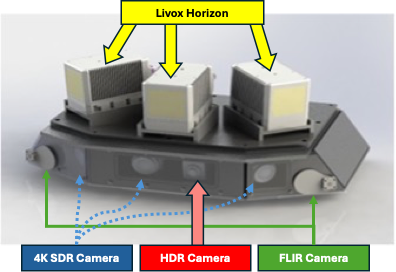
\includegraphics[width=0.8\textwidth]{Images/Camera_enclosure2.png}
\caption{Mounting locations of two LWIR cameras, three FLIR 4k cameras, and a single HDR camera within the camera enclosure, and three Livox Horizon LiDAR units affixed on top.}
\label{fig:camera_enclosure}
\end{figure}
        
\section{Perception Geometry} \label{perception_geometry}

While the Velodyne \ac{LiDAR} sensors provide comprehensive 360-degree environmental awareness for navigation and collision avoidance, the forward-facing Livox Horizon \ac{LiDAR} units were selected for their superior point cloud density and ability to facilitate a higher resolution for object detection.
The three Livox units concentrate sampling density in the forward field of view, matching the horizontal coverage of the six cameras.
Both modalities overlap the field of view of their respective individual sensors.
This sensor arrangement ensures higher density and more uniform point-cloud across the 165-degree forward perception envelope in the case of \ac{LiDAR}, but also makes the system more robust to failure.
Losing a single sensor will not create a blind spot for either sensing modality in the forward path of motion of the \ac{USV}. 
Figures~\ref{fig:fov_cam} and ~\ref{fig:fov_lidar} show how the horizontal \ac{FOV} for each of these sensors overlaps in the direction of travel.


\begin{figure}[htbp]
\centering
\begin{subfigure}[t]{0.45\textwidth}
    \centering
    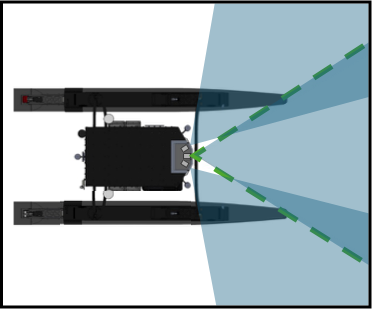
\includegraphics[width=\textwidth]{Images/fov_cam.png}
    \caption{Blue cones represent FOV from individual FLIR 4K camera; green dashed lines indicate FOV of HDR camera.}
    \label{fig:fov_cam}
\end{subfigure}
\hfill
\begin{subfigure}[t]{0.45\textwidth}
    \centering
    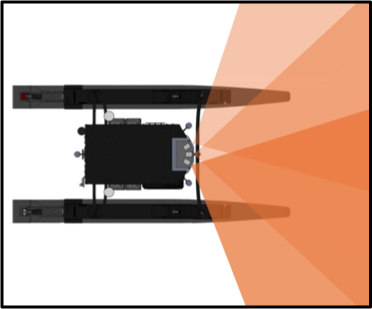
\includegraphics[width=\textwidth]{Images/fov_lidar.png}
    \caption{LiDAR horizontal FOV overlap.}
    \label{fig:fov_lidar}
\end{subfigure}
\caption{Comparative visualization of horizontal field of view (FOV) overlap for (a) cameras and (b) LiDAR sensors.}
\label{fig:fov_combined}
\end{figure}

A PinPoint \ac{GPS}/\ac{IMU} system provides both global time synchronization and platform pose estimation.

The sensor coordinate frames are organized in a hierarchical transformation tree structure.
The inertial reference frame (\texttt{map}) defines the world-fixed coordinate system based on \ac{GPS}.
The platform reference frame (\texttt{base\_link}) represents the vessel body frame defined by the PinPoint \ac{GPS}/\ac{IMU}.
The center Livox frame (\textcolor{red}{\texttt{livox\_center}}) serves as the primary \ac{LiDAR} reference, with the port Livox frame (\textcolor{red}{\texttt{livox\_port}}) and starboard Livox frame (\textcolor{red}{\texttt{livox\_starboard}}) as child frames.
Six camera image frames exist within this tree, with \textcolor{red}{camera frame} serving as the primary camera for fusion research.
Intrinsic calibration parameters, including camera-specific matrices and distortion coefficients, along with extrinsic transformation parameters relating sensor frames to each other and to the platform frame, are discussed in \textcolor{red}{Appendix \#}.

The Livox scan pattern employs a non-repetitive rosette pattern that progressively covers the field of view over time rather than repeatedly sampling fixed positions.
This characteristic enables temporal aggregation to increase effective spatial resolution, particularly beneficial for a moving platform where \ac{GPS}/\ac{IMU} pose data enables motion-compensated point cloud accumulation.

The dual \ac{LiDAR} architecture serves complementary purposes.
The Velodyne HDL-32E units provide the omnidirectional awareness required for autonomous navigation, while the Livox Horizon sensors optimize point cloud density specifically within the forward camera field of view for fusion research.
This configuration enables comparative evaluation of detection performance while maintaining operational navigation capabilities.
The sensor suite supports the research objectives of comparing detection performance across modalities and evaluating late fusion approaches.
The following subsections detail individual sensor specifications and selection rationale.

The primary sensors used for the data collected for this research were from the forward-facing perception module, referred to as the camera enclosure.


    \section{Sensors} \label{sensors}

This section details the technical specifications of the camera enclosure perception suite and discusses visual range sensor selection. 
The original sensor selection and configuration identified here was developed by \cite{thompson2023}, establishing a robust platform for maritime perception research. 
The primary enhancement introduced in this work is a timestamp embedding mechanism robust to network delay, detailed in Section~\ref{video pipeline}, which is essential for rigorous multi-modal sensor fusion analysis.

\subsection{LWIR Thermal Cameras} \label{sensors_LWIR}
Two Teledyne Calibir 640 \ac{LWIR} thermal cameras extend perception to night and low-light conditions. 
While limited to 640×480 resolution due to bolometer technology, they provide a combined 165-degree forward field of view when paired, ensuring redundancy with the
visible and HDR cameras.
textcolor{red}{Possibly remove this subsection?}

\subsection{Visible Spectrum Cameras} \label{sensors_cameras}

% \textcolor{red}{Expand this entire discussion}
The visible spectrum camera suite on the Minion platform is designed to balance two factors that are particularly important for maritime perception: imaging resolution and dynamic range.  

Camera resolution determines the ability to resolve small targets at a distance, and specific imaging sensors and lenses can be selected by determining the size and distance at which objects need to be resolved.
To ensure adequate object resolution across the operational envelope, cameras must resolve objects to a required resolution when the object is at the maximum detection range.

For an object of physical width $W$ at distance $d$, its width in the image frame $w_{\text{px}}$ is approximated by

  \begin{equation}
  w_{\text{px}} = \frac{f \, N_x \, W}{S_w \, d}
  \end{equation}

where $f$ is the \ac{EFL} of the camera and lens (mm), $N_x$ is the horizontal image resolution in pixels, and $S_w$ is the width of the image sensor (mm). 

% For the smallest target class (A-series buoys with a diameter $w_{\text{object}} = 0.61$~m) at maximum detection range $d = 60$~m, using the Blackfly S 4K specifications ($N_{\text{pixels}} = 4096$ pixels, $\theta_{\text{FOV}} = 65^\circ = 1.134$~rad), the expected pixel coverage is

%   \begin{equation}
%   n_{\text{pixels}} = \frac{0.61 \times 4096}{60 \times 1.134} \approx
%   36~\text{pixels}
%   \end{equation}

% This resolution exceeds the minimum requirement of approximately $10 - 15$ pixels for reliable object detection with modern convolutional neural networks, ensuring sufficient feature representation for classification even under degraded visibility conditions.
% The 4K sensor resolution was selected to maintain this margin across the entire perception envelope without requiring ultra-wide lenses that would introduce significant barrel distortion and reduce effective pixel density at range.

Defining these requirements requires an understanding of the object detection method used with visual cameras as well as the objects being detected, both of which will be discussed in greater detail in sections ~\ref{yolo} and ~\ref{dataset} respectively.
For now, it is sufficient to know that the smallest object we wish to detect is $0.3683$ meters wide at a distance of 60 meters, and that image detection scales each image frame down to a resolution of $\text{max}(640) \times \text{max}(640)$ pixels (preserving the original aspect ratio).
This means that an image captured at $4000 \times 3000$ pixels is reduced to $650 \times 487$ pixels, which is $16.25\%$ of its original size. 

This means that 

Consequently, if know that 
% Consequently, an object that appears to be 100 pixels wide in the image frame will be $16$ pixels wide when scaled down for the detection algorithm.

% Given a camera with horizontal resolution $N_{\text{pixels}}$ and horizontal field of view $\theta_{\text{FOV}}$, the angular resolution per pixel is

%   \begin{equation}
%   \theta_{\text{pixel}} = \frac{\theta_{\text{FOV}}}{N_{\text{pixels}}}
%   \end{equation}

% The number of pixels $n_{\text{pixels}}$ spanning the target object is therefore

%   \begin{equation}
%   n_{\text{pixels}} = \frac{\theta_{\text{object}}}{\theta_{\text{pixel}}} =
%    \frac{w_{\text{object}} \cdot N_{\text{pixels}}}{d \cdot
%   \theta_{\text{FOV}}}
%   \end{equation}





The dynamic range of an imaging sensor refers to the range of signal intensities it can detect, from the faintest signal that can be recorded to the brightest signal before saturation.
Insufficient dynamic range leads to washed-out highlights or lost detail in shadows.  
Because maritime environments routinely present both bright sky reflections and deep shadows in the same scene, dynamic range is as critical as resolution when selecting cameras for perception tasks.  

\subsubsection{FLIR Blackfly S 4K Cameras} \label{sensors_FLIR}

Three FLIR Blackfly S 4K visible-light cameras, arranged to provide a combined 165 degrees of forward-facing coverage through overlapping 65-degree lenses.  
As detailed in table \textcolor{red}{???}, This configuration avoids the distortion that would occur with fewer sensors equipped with ultra-wide lenses.
Each camera has a focal length of \textcolor{red}{???} and an image resolution of $4096 \times 4096$, ensuring that objects remain adequately resolved across the vessel's perception envelope.  
\begin{table}[htbp]
\centering
\caption{FLIR 4K Camera Specifications}
\begin{tabular}{ll}
\hline
\multicolumn{2}{c}{4K SDR Camera}\\
% HDR & Camera\\
\hline
% \textbf{Parameter} & \textbf{Value} \\
\hline
% Make & Leopard Imaging \\
FLIR & Blackfly S 120S4C \\
% Image Sensor & Sony IMX490 \\
% Pixel Size & $3.0 \times 3.0 \mu m$ \\
Horizontal Resolution & 4000 pixels \\
Vertical Resolution & 3000 pixels \\
Aspect Ratio & 1.33:1 \\
Maximum Frame Rate & 31 fps \\
Dynamic Range & 69.4 dB \\
\multicolumn{2}{c}{Camera Lens}\\
\hline
Theia & TL410P\\
% Aperture F/\# & $2.0$ \\
Horizontal \Ac{FOV} & 65-degrees\\
% Vertical Field of View & 37 degrees \\
\hline
\end{tabular}
\label{tab:SDR_camera_specs}
\end{table}

Each Blackfly S sensor achieves an effective dynamic range of 69.4~dB.  
% This corresponds to a span of a few thousand-to-one between the darkest detectable signal and the brightest non-saturating signal.  
The cameras capture 31 \ac{FPS} at a resolution of 4096 $\times$ 2160 pixels.
% \textcolor{red}{Add discussion of pixel density sensor selection in the context of the requirement to resolve specific objects at a minimum resolution at a maximum specific distance. This will require equations.}


\subsubsection{Leopard Imaging HDR Camera} \label{sensors_HDR}

A Leopard Imaging LI-USB30-IMX490-GW5400-GMSL2-065H camera, based on Sony’s IMX490 automotive-grade HDR sensor, provides 65 degrees of forward coverage.  
The camera delivers a resolution of 2880 $\times$ 1860 pixels at 25 frames per second.  
Most notably, the IMX490 achieves approximately 120~dB of dynamic range, extending the span of detectable light intensity to nearly one million-to-one.  

This performance is enabled by a digital overlap HDR (DOL-HDR) architecture with in-pixel dual conversion gain.  
By capturing multiple gain levels within a single frame period, the sensor produces simultaneous multi-gain readouts without relying on sequential multi-exposure stacking.  
This design eliminates ghosting and motion artifacts, which are common when either the platform or surrounding targets move between exposures.  

\subsubsection{HDR Selection}

The FLIR Blackfly S 4K cameras satisfy geometric and resolution requirements, but their limited dynamic range makes them prone to over-exposure and loss of highlight detail in high-contrast maritime conditions. 
They support an effective dynamic range of 69.4~dB, which corresponds to a span of just a few thousand-to-one between the darkest detectable signal and the brightest non-saturating signal. 
As a result, the cameras are prone to over-exposure in high-brightness maritime conditions, particularly when imaging reflective water surfaces or bright sky backgrounds, leading to loss of highlight detail and reduced contrast. 

In contrast, the IMX490 HDR camera combines a comparable field of view with substantially greater dynamic range, enabling detail preservation across bright and shaded regions within the same frame.  
For these reasons, the HDR camera was designated as the primary forward-facing visual spectrum sensor for \ac{LiDAR}-camera fusion research.  
 
As a result, the cameras are prone to over-exposure in high-brightness maritime conditions, particularly when imaging reflective water surfaces or bright sky backgrounds, leading to loss of highlight detail and reduced contrast.  

These limitations highlighted the need for a true high-dynamic-range (HDR) sensor to complement the Blackfly cameras.  
 

\subsubsection{Leopard Imaging HDR Camera}

To overcome these limitations, a Leopard Imaging LI-USB30-IMX490-GW5400-GMSL2-065H camera was integrated, based on Sony’s IMX490 automotive-grade HDR sensor.  
This camera provides 65 degrees of forward coverage and achieves approximately 120~dB of dynamic range, enabling preservation of fine image details across extreme lighting conditions, including bright sky, reflective water, and shaded objects.  

The IMX490 accomplishes this performance using a digital overlap HDR (DOL-HDR) architecture with in-pixel dual conversion gain.  
This method captures multiple effective exposures within a single frame period, producing simultaneous multi-gain readouts from the same scene.  
Unlike sequential multi-exposure HDR, which stacks separate frames and is prone to ghosting or blurring, DOL-HDR eliminates motion artifacts—a critical capability in maritime operations where both the vessel and surrounding objects are frequently in motion.  

This substantial increase in dynamic range, combined with robust performance under challenging illumination, made the IMX490-based HDR camera the primary visual spectrum sensor for \ac{LiDAR}-camera fusion research in this dissertation.  
Preliminary results from a comparative study by Liebergall et al.~\cite{liebergall} further supported this decision, showing improved detection consistency with the HDR sensor compared to the FLIR 4K cameras.  
Although later published results did not fully corroborate the preliminary findings, those results became available only after the dataset for this research had been collected.  
Accordingly, the IMX490 HDR camera served as the main forward-facing visual spectrum sensor throughout this study.  

\begin{table}[htpb]
\centering
\caption{HDR Camera Specifications}
\begin{tabular}{ll}
\hline
\multicolumn{2}{c}{HDR Camera}\\
% HDR & Camera\\
\hline
% \textbf{Parameter} & \textbf{Value} \\
\hline
% Make & Leopard Imaging \\
Leopard Imaging & LI-IMX490-GW5400-GMSL2-065H \\
Image Sensor & Sony IMX490 \\
Pixel Size & $3.0 \times 3.0 \mu m$ \\
Horizontal Resolution & 2880 pixels \\
Vertical Resolution & 1860 pixels \\
Aspect Ratio & 1.55:1 \\
Maximum Frame Rate & 25 fps \\
Dynamic Range & 120 dB \\
Lens \Ac{EFL} & $7.9 mm$\\
Aperture F/\# & $2.0$ \\
\Ac{FOV} & 65-degrees (H), 37-degrees (V) \\
% Vertical Field of View & 37 degrees \\
\hline
\end{tabular}
\label{tab:hdr_camera_specs}
\end{table}

The 2880×1860 resolution provides sufficient spatial detail for detecting objects at relevant ranges in autonomous vessel navigation, while the 25 fps frame rate adequately supports typical vessel speeds and maneuvering.

The IMX490's native \ac{HDR} combines multiple exposures in a single frame period, achieving 120 dB dynamic range without sequential multi-exposure capture.
This simultaneous approach eliminates motion artifacts associated with temporal bracketing, which is critical when both the platform and targets are in motion.
Image quality validation and intrinsic calibration are addressed in Section 3.2.1.1, including lens distortion characterization and camera matrix estimation.
The combination of wide dynamic range, moderate resolution, and calibrated geometry provides the image quality necessary for training and evaluating vision-based detection models in Chapter 5.

Thompson et al. \cite{thompson2023} originally developed this camera hardware and integration approach, establishing a foundation for maritime perception research.
The primary enhancement introduced in this work comprises in-band timestamp embedding and temporal drift correction, detailed in Section 3.2.2, which are essential for rigorous multi-modal sensor fusion analysis.

        \subsection{LiDAR Systems} \label{sensors_LiDAR}

The Minion platform features six \ac{LiDAR} units providing both omnidirectional environmental awareness and forward-facing high-density perception.
The \ac{LiDAR} suite comprises three Velodyne HDL-32E units and three Livox Horizon units.

The three Velodyne HDL-32E mechanically rotating 360-degree \ac{LiDAR} sensors are positioned to provide complete omnidirectional point cloud coverage.
One unit is positioned at aft-center, with the other two placed at approximately one-third intervals around the vessel at forward-port and forward-starboard locations to achieve a full 360-degree field of view coverage.

The three Livox Horizon solid-state forward-scanning \ac{LiDAR} sensors provide high-density returns within a 165-degree forward field of view matching the camera array coverage.
These sensors were selected specifically for \ac{LiDAR}-camera fusion research based on superior point cloud density within the camera field of view and a non-repetitive scan pattern that enhances coverage through temporal aggregation \cite{thompson2023}.

% Initial planning considered utilizing the Velodyne HDL-32E sensors already installed on the Minion platform for fusion research.
% However, analysis of point cloud density within the camera field of view revealed fundamental limitations of mechanically rotating \ac{LiDAR} for sensor fusion applications.
% Traditional spinning sensors like the Velodyne HDL-32E employ a fixed vertical array of laser emitters that rotates horizontally at constant speed.
% The HDL-32E incorporates 32 laser channels arranged vertically across approximately 40 degrees of elevation.
% This array rotates at 10 Hz, producing 32 discrete horizontal rings of returns distributed across the full 360-degree plane \cite{thompson2023}.

While 360-degree coverage provides comprehensive spatial awareness, it presents challenges for camera-\ac{LiDAR} fusion.
First, sparse azimuthal sampling occurs because on a stationary or slow-moving platform, the 32 lasers strike identical positions on every rotation, yielding no increase in sampling density over time.
Second, inefficient field of view utilization results from distributing returns across 360 degrees, such that only a fraction falls within the forward-facing camera view.
These limitations motivated the selection of an alternative \ac{LiDAR} technology optimized for forward-facing perception with temporal aggregation.

The Livox Horizon employs a non-repetitive rosette scan pattern that progressively covers its field of view over time rather than repeatedly sampling identical locations.
The sensor features an 81.7-degree × 25.1-degree (horizontal × vertical) field of view, substantially wider in azimuth than the 65-degree cameras.
Three Livox units deployed together achieve a combined coverage of approximately 165 × 25.1 degrees, providing complete horizontal overlap with the camera array and covering approximately 77\% vertically \cite{thompson2023}.
Table 3.2 presents the Livox Horizon specifications.

\begin{table}[htpb]
\centering
\caption{LiDAR Specifications}
\begin{tabular}{ll}
\hline
\multicolumn{2}{c}{Livox Horizon}\\
\hline
% \textbf{Parameter} & \textbf{Value} \\
\hline
Model & Livox Horizon \\
Horizontal Field of View & 81.7 degree \\
Vertical Field of View & 25.1 degree \\
Range & 260 m @ 80\% reflectivity \\
Point Rate (Single Return) & 240,000 pts/sec \\
Point Rate (Dual Return) & 480,000 pts/sec \\
Range Precision & ±2 cm \\
Wavelength & 905 nm \\
Scan Pattern & Non-repetitive rosette \\
Interface & Ethernet \\
Operating Frequency & 100 Hz \\
\hline
\end{tabular}
\label{tab:livox_horizon_specs}
\end{table}

The 905 nm near-infrared wavelength experiences strong absorption by water, resulting in minimal returns from water surfaces.
This characteristic benefits maritime object detection by reducing clutter from waves that would otherwise trigger false positives in clustering algorithms.

The fundamental distinction between the Livox Horizon and traditional spinning \ac{LiDAR} lies in the scan pattern.
A mechanically spinning sensor with N lasers produces N discrete horizontal rings that repeat identically each rotation.
For vessels moving at typical speeds (2-5 m/s), platform displacement between rotations remains small relative to object size, resulting in near-perfect overlap of consecutive scans.
The Livox operates differently, employing a two-dimensional scanning mechanism that traces a non-repetitive rosette pattern across the field of view.
Two orthogonal mirrors operating at slightly different frequencies cause the laser beam to trace a complex Lissajous-like path that progressively fills the field of view without repetition \cite{thompson2023}.

Scan pattern coverage accumulates over time, with longer integration periods yielding denser spatial sampling.
At the standard 100 Hz output rate, each \ac{UDP} message contains approximately 10 milliseconds of returns.
Over a one-second aggregation period, the rosette pattern provides substantially higher spatial coverage than a spinning sensor's fixed ring geometry.

The non-repetitive forward-scanning nature of the Livox units means that point cloud density is not uniform across the field of view.
The 81.7-degree horizontal field of view allows for overlap between the three units, achieving more uniform density across the 165-degree field of view, matching the 4K FLIR camera coverage.

% Insert figure showing Livox scan pattern here
\begin{figure}[htbp]
\centering
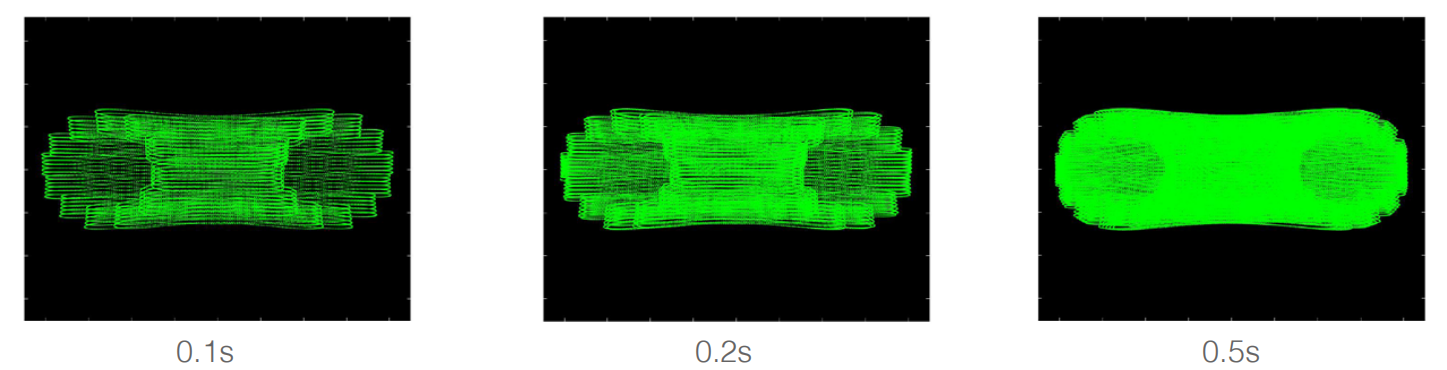
\includegraphics[width=0.8\textwidth]{Images/Livox_1.png}
\caption{Livox Horizon non-repetitive rosette scan pattern demonstrating point cloud density distribution from 0.1 to 0.5 seconds.}
\label{fig:livox_scan_pattern}
\end{figure}

Figure \ref{fig:livox_scan_pattern} illustrates the non-repetitive rosette scan pattern and resulting point cloud density distribution.
This density is critical for the grid-based clustering employed for \ac{LiDAR} object detection in Chapter 5.

Comparison of point cloud density within the camera field of view reveals the Livox advantage.
A Velodyne HDL-32E in dual-return mode produces approximately 1.4 million points per second distributed across the full 360-degree plane.
The camera field of view encompasses approximately 165 degrees, yielding an effective point rate in the region of interest of:

$$\text{Effective HDL-32E rate} = 1.4 \times 10^6 \times \frac{165 degree}{360 degree} \approx 641,000 \text{ pts/sec}$$

Three Livox Horizon units in dual-return mode together produce:

$$\text{Combined Livox rate} = 3 \times 480,000 = 1.44 \times 10^6 \text{ pts/sec}$$

This represents a 2.25× increase in point returns within the camera view, excluding additional benefits from superior vertical sampling achieved through the non-repetitive pattern compared to fixed 32-ring geometry \cite{thompson2023}.

The non-repetitive scan pattern demonstrates particular advantage when aggregating multiple scans over time, accumulating points over an integration window to enhance spatial sampling.
On a moving platform, motion compensation during the accumulation period becomes necessary.
The \ac{LiDAR} aggregation approach, detailed in Chapter 5, employs the \ac{GPS}/\ac{IMU} to track platform pose over time.
Each \ac{LiDAR} point is transformed from sensor coordinates to a world reference frame using the platform pose at that point's timestamp.
All accumulated points are then transformed from world coordinates to the target camera image frame, enabling overlay of a dense point cloud on the image.
A four-second integration period was selected based on empirical evaluation of the tradeoff between point cloud density and motion blur.
Each camera image sampled at 1 Hz receives all \ac{LiDAR} points from the preceding four seconds, transformed to the image capture time.
This approach provides the spatial resolution necessary for reliable detection while maintaining sufficient motion compensation accuracy for typical vessel speeds.

The Livox Horizon sensors communicate via \ac{UDP} over Ethernet, transmitting point cloud data as binary messages at 100 Hz.
Livox provides an open-source \ac{ROS} SDK that manages network communication, message parsing, and point cloud publication to \ac{ROS} topics.
Integration of the Livox SDK into the Minion software required minimal effort, primarily involving network configuration and modification of \ac{ROS} launch files.
The SDK operates on the Atlas PC, receiving \ac{UDP} messages from all three \ac{LiDAR} units simultaneously over the local network described in Section 3.1.2.3.

Accurate fusion of data from multiple \ac{LiDAR} units requires precise knowledge of sensor geometric relationships.
The Livox Horizon units feature onboard storage for extrinsic calibration parameters, enabling each sensor to transform its measurements to a common reference frame before transmission.
The \ac{LiDAR}-to-\ac{LiDAR} extrinsic calibration presented in Section 3.2.1.3 determines the six-degree-of-freedom transformation (translation and rotation) relating each sensor's local coordinates to the designated primary sensor.
These parameters are written to non-volatile memory on each Livox unit, configuring automatic application of the transformation such that all point clouds emerge in the center \ac{LiDAR}'s reference frame \cite{thompson2023}.
This onboard configuration simplifies downstream processing by eliminating the need for software-based registration of the three point clouds.
The unified cloud is subsequently related to camera coordinates through camera-to-\ac{LiDAR} extrinsic calibration described in Section 3.2.1.2.

Temporal alignment of \ac{LiDAR} with camera images and \ac{GPS}/\ac{IMU} pose requires all \ac{LiDAR} points to possess timestamps referenced to a common global time base.
The Livox Horizon supports IEEE 1588 Precision Time Protocol, providing sub-microsecond clock synchronization with a \ac{PTP} master on the network.
In this configuration, the NVIDIA Jetson Xavier in the camera box functions as the \ac{PTP} master, synchronizing the three \ac{LiDAR} units.
The Jetson itself synchronizes to \ac{GPS} time via the Network Time Protocol hierarchy detailed in Section 3.2.2.1.
This cascaded synchronization ensures \ac{LiDAR} timestamps share the same \ac{GPS}-disciplined time reference as camera frames, enabling frame-accurate alignment for fusion.
\ac{PTP} synchronization status is verified using the Livox Viewer software, which displays sync state and time source for each sensor.
Proper \ac{PTP} lock is confirmed prior to data collection, ensuring timestamp accuracy.

An advantageous characteristic of the 905 nm wavelength is its strong absorption by water.
This results in minimal \ac{LiDAR} returns from water surfaces, contrasting with vision sensors that clearly image water texture and waves.
Absence of water returns reduces point cloud clutter and simplifies object detection by eliminating the need to filter ground plane points for the water surface.
Point cloud visualizations overlaid on camera images demonstrate this characteristic: dense \ac{LiDAR} coverage appears on vessels, buoys, and other solid objects, while water surfaces produce few or no returns.
For grid-based clustering, this characteristic prevents false positives from wave crests or foam patterns.

The Livox Horizon configuration provides several capabilities essential for comparing object detection performance.
The system achieves 2.25× more points within the camera view compared to omnidirectional spinning sensors, while the non-repetitive scan pattern enhances sampling density through temporal aggregation.
Per-point timestamps and \ac{GPS}/\ac{IMU} integration enable accurate aggregation during motion, while \ac{PTP} synchronization provides sub-microsecond timing accuracy relative to cameras and \ac{GPS}.
Factory-configured multi-sensor calibration unifies point clouds from three sensors before transmission, and the 905 nm wavelength reduces maritime clutter by rejecting water returns.
Combined with the software integration and synchronization infrastructure described in Section 3.2, this configuration enables rigorous \ac{LiDAR} detection evaluation and comparison with vision-based approaches in Chapters 5 and 6.

        \subsection{PinPoint GPS/INS} \label{sensors_GPS}

The Minion platform features a single PinPoint \ac{GPS}/\ac{IMU} with differential corrections.
The system performs two critical functions in the perception architecture: providing precise global time for sensor synchronization, and tracking vessel position and orientation for motion correction of \ac{LiDAR} data.
The \ac{GPS} receiver functions as the master clock for the entire synchronization hierarchy described in Section 3.2.2.1, while the integrated \ac{IMU} enables high-rate pose updates between \ac{GPS} fixes.

Global Navigation Satellite System signals inherently carry highly accurate timing information, as satellite positioning operates through precise measurement of signal delay from multiple satellites with synchronized atomic clocks.
The PinPoint receiver extracts this timing information and distributes it over the vessel's network using Network Time Protocol.
The \ac{GPS} unit was assigned a static IP address of 201.7.90.30 on the Minion network and configured to broadcast \ac{GPS}-disciplined time via Network Time Protocol.
The Atlas PC main computer synchronizes its clock to this \ac{GPS} source with typical accuracy in the tens to hundreds of nanoseconds, limited primarily by network latency rather than \ac{GPS} accuracy.

This \ac{GPS} time reference propagates through the synchronization hierarchy to every computing resource on the platform.
Atlas functions as a Network Time Protocol server for the NVIDIA Jetson Xavier camera computer, which subsequently operates as a Precision Time Protocol master for the Livox Horizon \ac{LiDAR} sensors.
This cascaded approach ensures timestamps from all sensors—cameras, \ac{LiDAR}, and \ac{GPS}/\ac{IMU}—share a common time reference traceable to \ac{GPS} time.

Beyond timekeeping, the \ac{GPS}/\ac{IMU} system continuously tracks platform position and orientation, which is required for \ac{LiDAR} temporal aggregation.
As described in Section 3.1.1.3, accumulating \ac{LiDAR} points over several seconds necessitates compensation for vessel motion during that period.
The PinPoint system fuses \ac{GPS} position measurements with \ac{IMU} acceleration and rotation data through an Extended Kalman Filter to produce pose estimates at rates substantially higher than \ac{GPS} alone could provide.
\ac{GPS} fixes arrive at 1-10 Hz depending on satellite visibility, while the \ac{IMU} operates at hundreds of hertz.
The fusion algorithm propagates pose estimates forward using \ac{IMU} integration between \ac{GPS} updates, subsequently correcting accumulated drift when new \ac{GPS} measurements arrive.

The resulting pose solution provides six-degree-of-freedom state estimates—three-dimensional position and three-dimensional orientation—at sufficient temporal resolution to interpolate platform pose to the exact timestamp of each \ac{LiDAR} point.
This capability supports the transformation methodology presented in Chapter 5, where \ac{LiDAR} points acquired at different times during motion are transformed to a common reference frame before projection onto camera images.

The PinPoint \ac{GPS}/\ac{IMU} connects to the Minion computing infrastructure via Ethernet, utilizing both Network Time Protocol for time distribution and User Datagram Protocol for pose data transmission.
\ac{ROS} driver nodes on the Atlas PC receive and parse the binary \ac{GPS}/\ac{IMU} messages, publishing pose estimates as standard \ac{ROS} geometry messages.
These messages incorporate position (latitude, longitude, altitude), orientation (roll, pitch, yaw), uncertainty estimates, and \ac{GPS} fix quality flags.
The \ac{ROS} tf2 library consumes these pose estimates to maintain the time-varying transformation tree relating sensor frames to platform and world frames, enabling automated coordinate transformation for sensor fusion.

The \ac{GPS}/\ac{IMU} defines the inertial reference frame for the platform, with position expressed in geographic coordinates (WGS84 datum) and orientation relative to true north and local gravity.
This world-referenced system serves as the common reference for transforming observations from multiple sensors acquired at different times during motion.
Transformation from sensor-local frames to the \ac{GPS}/\ac{IMU} world frame requires knowledge of sensor-to-platform extrinsic calibration parameters.
These parameters are determined through calibration procedures described in Section 3.2.1.2 for cameras and Section 3.2.1.3 for \ac{LiDAR} sensors.
With extrinsic parameters established, the \ac{GPS}/\ac{IMU} pose solution enables transformation of any sensor observation to world coordinates or to any other sensor's reference frame.

Maritime environments present challenges for \ac{GPS}/\ac{IMU} systems that differ from land vehicle applications.
Water surface reflections induce multipath interference in \ac{GPS} signals, while vessel pitch and roll motion exercises the full range of the \ac{IMU}.
The PinPoint system was designed for marine applications and incorporates algorithms to address these factors while maintaining accuracy during vessel maneuvering.
\ac{GPS} accuracy degrades in areas with limited satellite visibility, such as proximity to tall structures, bridges, or fjord-like coastal terrain.
The \ac{IMU} provides short-term pose continuity during \ac{GPS} outages, though accumulated drift limits the duration for which pure inertial navigation remains accurate.
Data collection operations were conducted in open water with favorable satellite visibility, ensuring consistent \ac{GPS} fix quality throughout recording sessions.

The \ac{GPS}/\ac{IMU} system enables two functions essential for multi-modal sensor fusion research.
First, \ac{GPS}-disciplined time distributed to all sensors ensures timestamps from cameras, \ac{LiDAR}, and \ac{GPS} itself reference the same time base, providing frame-accurate temporal association across modalities.
Second, continuous pose estimates enable transformation of temporally distributed observations to common reference frames, supporting \ac{LiDAR} aggregation during motion and registration of sensor fields of view for fusion operations.
Combined with the synchronization verification and drift correction procedures described in Section 3.2.2, these capabilities establish the temporal and spatial foundation for rigorous object detection performance evaluation across sensing modalities.
The \ac{GPS}/\ac{IMU} thus functions not merely as a navigation sensor but as critical infrastructure enabling the multi-modal perception analysis central to this research.

\subsection{Sensor Transforms}
The multi-sensor system aboard the WAM-V requires rigorous coordinate frame transformations to fuse data from heterogeneous sensors into a unified representation. Each sensor operates in its native coordinate frame, necessitating extrinsic calibration to establish spatial relationships between sensors and the vessel's body frame.

The fundamental transformation between coordinate frames is expressed as:
\begin{equation}
^Bp =\; ^B_AR \; ^Ap + ^B_A T
\end{equation}
where points in reference frame $A$ ($^Ap$) are transformed into reference frame $B$ ($^Bp$) through a rotation matrix $^B_AR$ and translation vector $^B_A T$.

% \subsubsection{Coordinate Frame Definitions}
The selected sensors employ multiple coordinate frames, each with distinct conventions:

% \textbf{Inertial Frame (Map):} 
The global reference frame follows the North-East-Down (NED) convention, where the x-axis points north, y-axis points east, and z-axis points downward toward the earth's center. This right-handed frame provides a consistent world reference for navigation and localization.

% \textbf{LiDAR Frame:} 
The Livox Horizon sensors capture point cloud data in the Forward-Left-Up (FLU) convention, where x-axis points forward along the sensor's optical axis, y-axis points left, and z-axis points upward. Each of the three LiDAR units maintains this local frame relative to its mounting position.

% \textbf{GPS Frame:} 
The GPS receiver outputs position data in geodetic coordinates (latitude, longitude, altitude), which are converted to Cartesian coordinates in the FLU body frame using the vessel heading from the inertial measurement unit (IMU). This transformation accounts for the spherical earth geometry and local tangent plane approximation.

% \textbf{Camera Frame:} 
The Leopard Imaging camera operates in a standard image plane coordinate system where the u-axis (horizontal) points right, v-axis (vertical) points down, and the optical axis extends forward along the camera's line of sight. Image coordinates require both extrinsic transforms to the body frame and intrinsic camera calibration for 3D reconstruction.

The sensor-to-body and body-to-inertial transformations are all handled through the \Ac{ROS} robot-localization package onboard the \Acp{USV} main computer, Atlas.
%%%%%%%%%%%%%%%%%%%%%%%%%%%%%%
\begin{figure}[htbp]
\centering
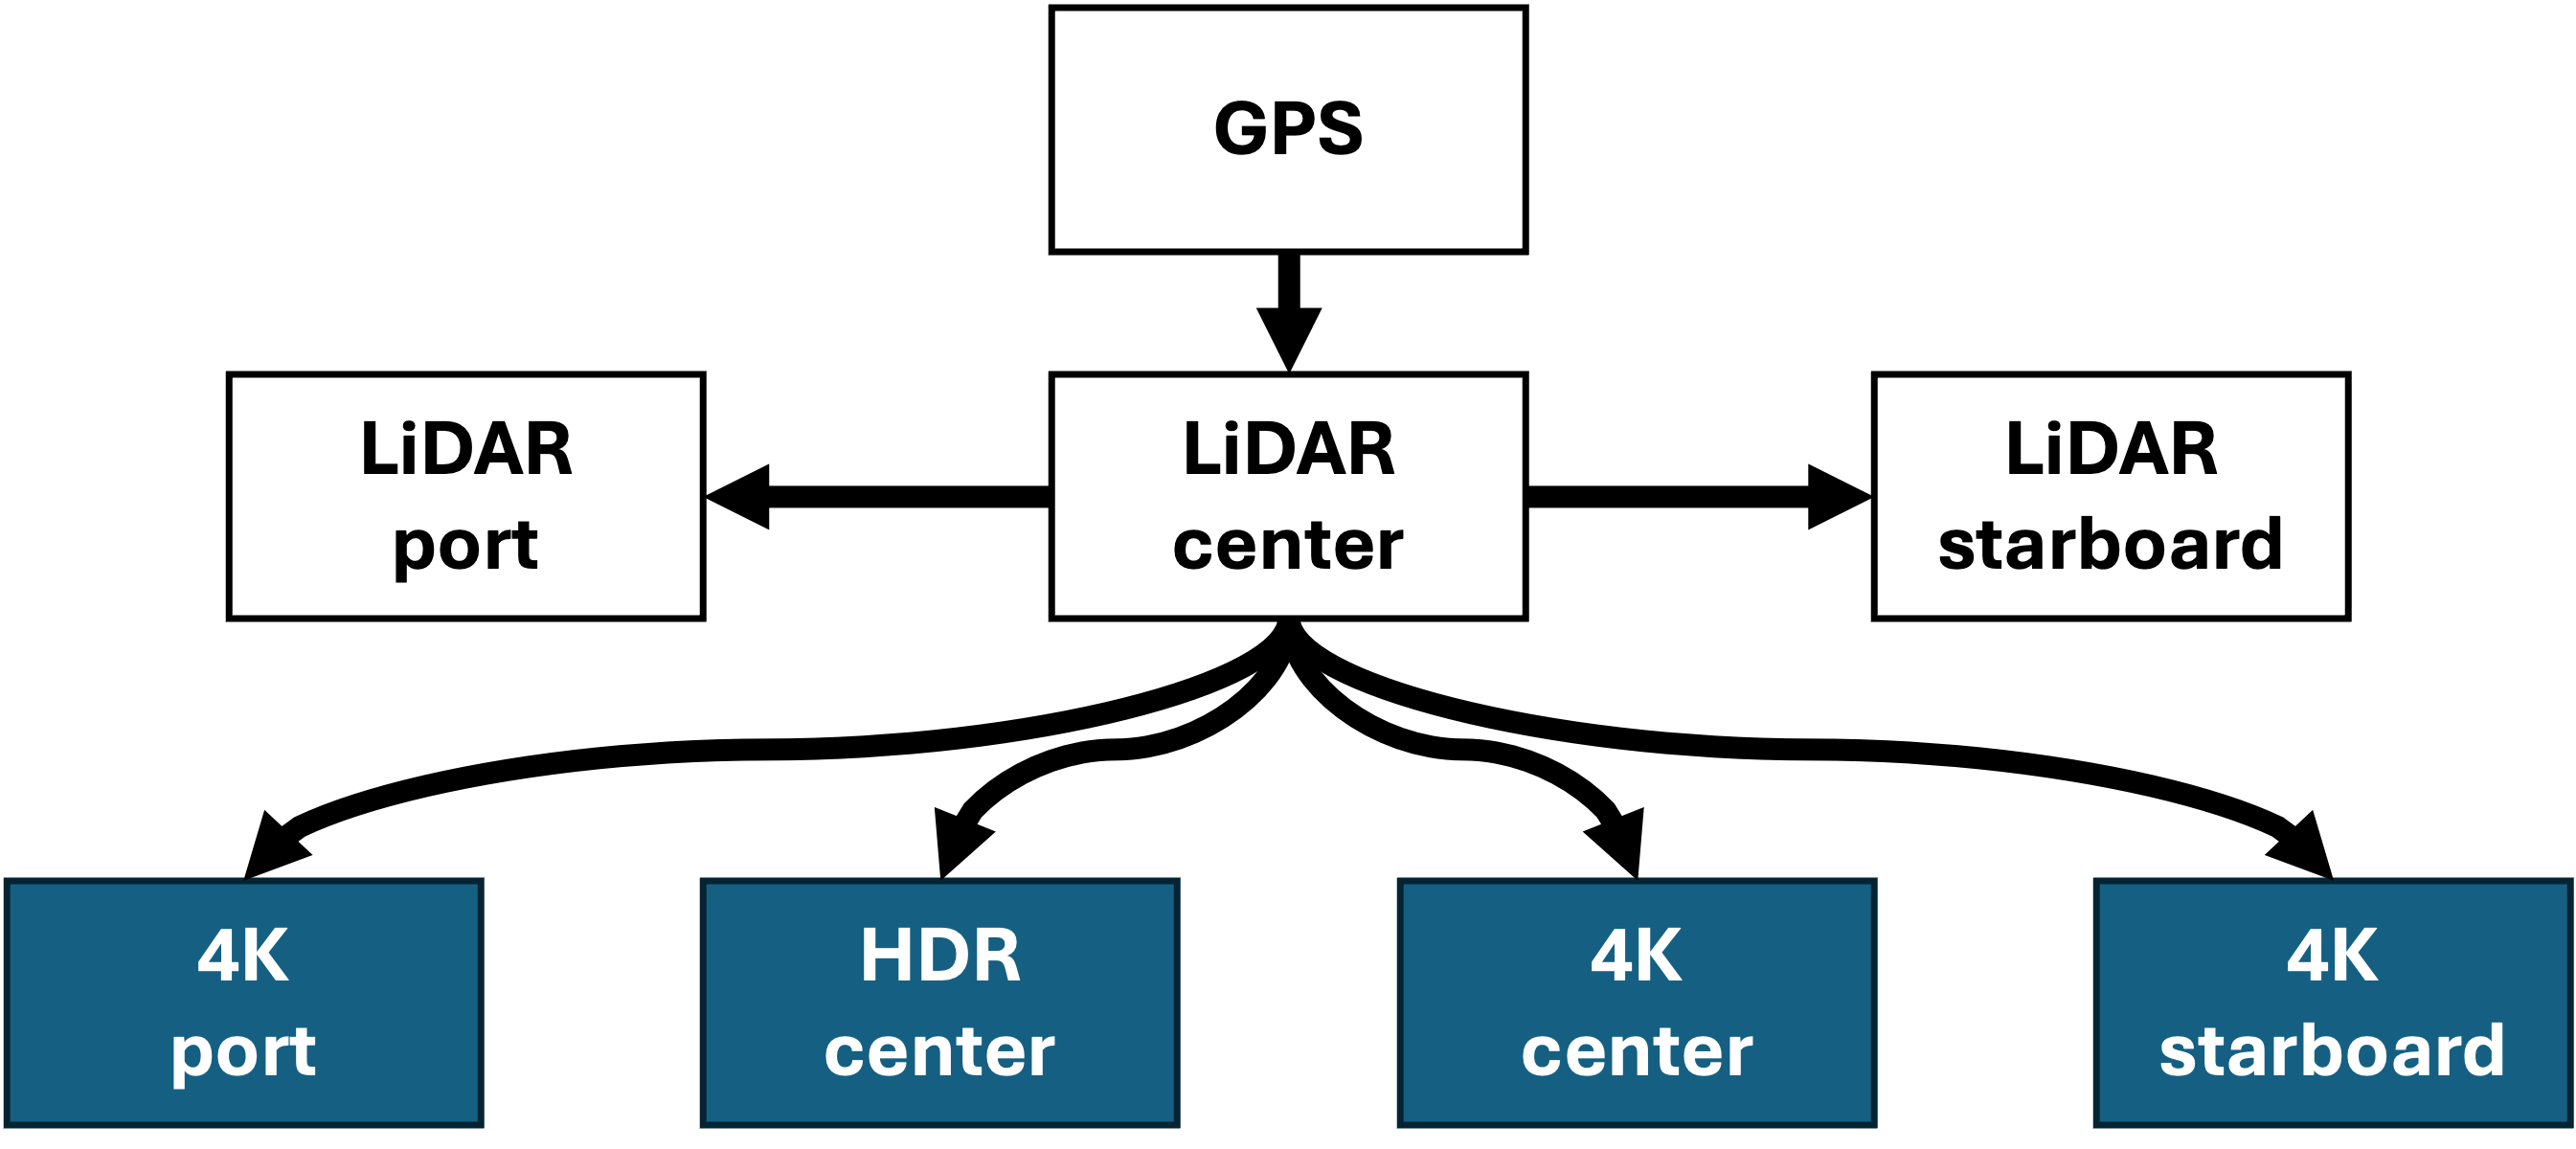
\includegraphics[width=0.75\textwidth]{Images/spatial_transforms.png}
\caption{A flowchart of transforms between sensor reference frames. Arrows indicate extrinsic transformations, and dark boxes indicate an additional intrinsic transform.}
\label{transform_diagm}
\end{figure}
%%%%%%%%%%%%%%%%%%%%%%%%%%%%%%

\section{Compute and LAN} \label{compute_lan}

The Minion platform's computing architecture consists of two primary systems: a main compute module housed in a waterproof Pelican case and a dedicated camera enclosure with integrated processing. The main compute module contains the Atlas PC and a 16-port network switch that aggregates all sensor and subsystem connections. The camera enclosure integrates a self-contained computing system responsible for camera data acquisition, video encoding, and timestamp synchronization with the vessel's global time reference. This modular architecture enables independent development and testing of the perception system while maintaining compatibility with the broader platform infrastructure.

\subsection{Camera Enclosure Computing Platform} \label{jetson_platform}

An NVIDIA Jetson AGX Xavier serves as the dedicated computer within the camera enclosure, handling all camera interface, video encoding, and network streaming operations. The Jetson was selected for its GPU acceleration capabilities, compact form factor, and native support for industrial camera interfaces including GMSL2 (Gigabit Multimedia Serial Link) required by the Leopard Imaging HDR camera.

The Jetson AGX Xavier features an 8-core ARM CPU, 512-core Volta GPU with 64 Tensor cores, and 32 GB of unified memory, providing sufficient computational resources for real-time video encoding of multiple simultaneous camera streams. The integrated GPU enables hardware-accelerated H.264/H.265 video encoding, reducing CPU load and network bandwidth requirements compared to uncompressed image transmission.

The Jetson connects directly to all cameras within the enclosure: the Leopard Imaging HDR camera via GMSL2 interface and three FLIR Blackfly S cameras via GigE Vision over Ethernet. Custom \ac{ROS} driver nodes execute on the Jetson to interface with each camera, configure acquisition parameters, capture frames, embed timestamps, encode video streams, and transmit encoded data to the vessel's main computer.

% A critical function of the Jetson platform is timestamp embedding for temporal synchronization. As described in Section~\ref{temporal_sync}, accurate sensor fusion requires camera frame timestamps to represent the actual moment of image capture referenced to a global time base. The Jetson system clock synchronizes to the vessel's \ac{GPS}-disciplined time reference via Network Time Protocol, then embeds synchronized timestamps into each video frame as supplemental encoded information (SEI) data within the H.264 stream. This approach ensures frame timestamps remain associated with image data throughout network transmission and decoding.

The camera enclosure design emphasizes modularity and research flexibility. The self-contained Jetson computer with local camera connections enables the perception system to be removed, modified, and tested independently of the Minion platform. Firmware updates, camera reconfiguration, and software development can proceed in the laboratory without requiring access to the full vessel. Network connectivity to the Minion platform occurs through a single Ethernet connection carrying both encoded video streams via \ac{RTP} and bidirectional \ac{NTP} for clock synchronization.

\subsection{Network Architecture} \label{network_structure}

% The Minion platform implements a hierarchical local area network (LAN) architecture connecting all computing resources and sensors. The network topology separates high-bandwidth sensor data streams from lower-rate command and control traffic while maintaining deterministic latency for time-critical communications.

The Atlas PC functions as the central computing node, hosting the primary \ac{ROS} environment, object detection algorithms, mission planning software, and data logging infrastructure. Atlas connects to the vessel LAN via a gigabit Ethernet switch that aggregates connections from all network-capable sensors and subsystems.

% Key network endpoints include:
% \begin{itemize}
% \item \textbf{Jetson AGX Xavier} (camera enclosure): Video streams and timestamp synchronization
% \item \textbf{Livox Horizon \ac{LiDAR} units} (3 sensors): UDP point cloud data at 100 Hz per sensor
% \item \textbf{PinPoint \ac{GPS}/\ac{IMU}}: Pose data and Network Time Protocol time reference
% \item \textbf{Velodyne HDL-32E \ac{LiDAR} units} (3 sensors): UDP point cloud data for navigation
% \item \textbf{Shore connection}: Ground station monitoring and remote access during development
% \end{itemize}

Static IP address assignment ensures deterministic routing and simplifies network administration. The PinPoint \ac{GPS}/\ac{IMU} is configured with IP address 201.7.90.30 and designated as the authoritative Network Time Protocol server for the vessel. All other computing resources synchronize to this \ac{GPS}-disciplined time source to establish a common temporal reference.

This \ac{RTP}-based approach was developed to address network latency issues observed with alternative solutions. Open-source plugins such as GStreamer-based GSCam and NVIDIA's DeepStream SDK were evaluated but found insufficient for Minion's specific requirements. The custom implementation provides granular control over video encoding parameters (resolution, frame rate, bitrate, compression method) and ensures embedded timestamps survive the encoding-transmission-decoding pipeline without modification.

Point cloud data from the three Livox Horizon \ac{LiDAR} sensors arrives as \ac{UDP} packets transmitted directly to the Minion LAN at 100 Hz per sensor. The Livox SDK executing on Atlas receives these streams, parses binary point cloud messages, and publishes data to \ac{ROS} topics for consumption by perception algorithms. 

\begin{figure}[htbp]
    \centering
    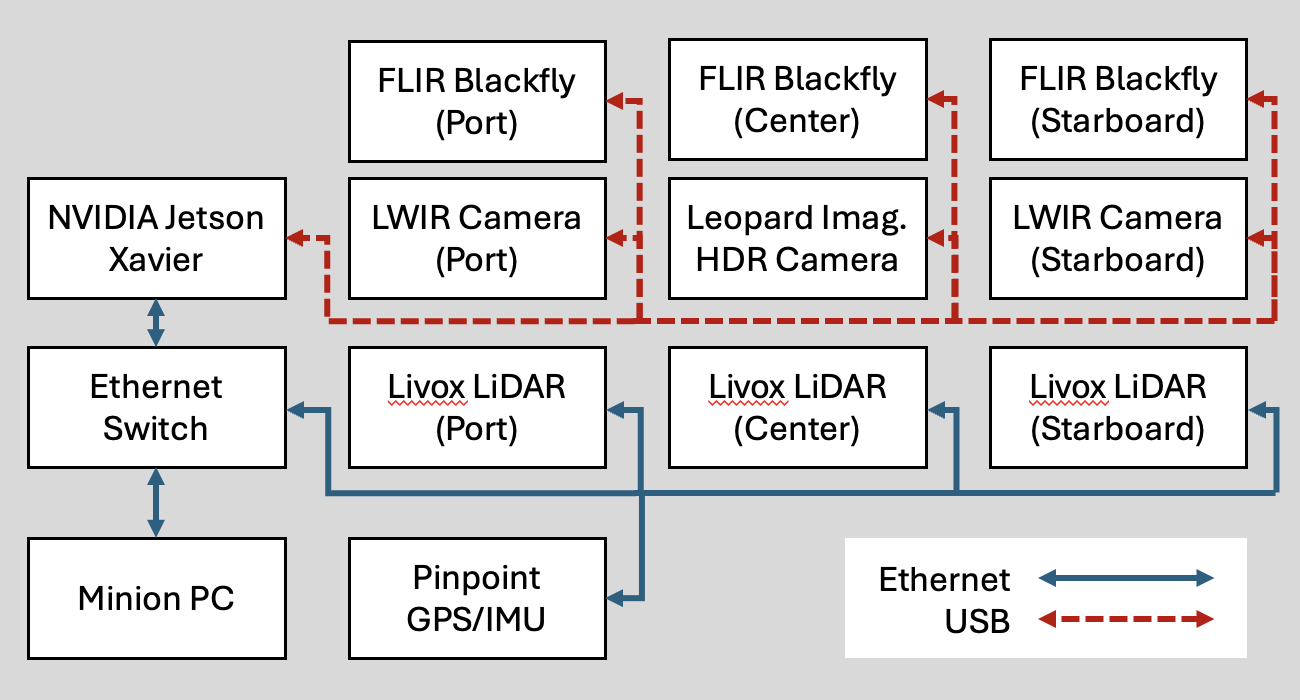
\includegraphics[width=0.85\textwidth]{Images/network_diagram.png}
    \caption{Block diagram of the network architecture of the \ac{USV}. Red dashed arrows indicate USB connections and blue solid arrows indicate Ethernet-connected blocks.}
    \label{fig:network_diag}
\end{figure}

Bandwidth analysis for the forward perception system indicates peak data rates of approximately:

\begin{table}[htbp]
\centering
\caption{Peak data rates for forward perception sensors}
\label{tab:network_bandwidth}
\begin{tabular}{lccc}
\hline
\textbf{Sensor} & \textbf{Specifications} & \textbf{Quantity} & \textbf{Data Rate} \\
\hline
Livox \ac{LiDAR} & 480k pts/sec, dual return, 100 Hz, 16 bytes/pt & 3 & $\approx$ 23 Mbps \\
HDR Camera & H.264, 5 fps, 2880$\times$1860 & 1 & 8--12 Mbps \\
% FLIR Cameras & H.264, 31 fps, 4000$\times$3000 & 3 & 15--25 Mbps each \\
\hline
\end{tabular}
\end{table}

Total sustained network load during perception operations remains well below the gigabit Ethernet capacity, ensuring minimal packet loss and deterministic latency.

Quality of Service (QoS) configuration prioritizes time-sensitive traffic such as \ac{GPS}/\ac{IMU} pose updates and Network Time Protocol synchronization packets over bulk data transfers. This ensures clock synchronization accuracy is maintained even during periods of high sensor data throughput.

The hierarchical network architecture with segregated sensor and control traffic, static addressing for deterministic routing, and low-latency \ac{UDP}-based protocols establishes a robust foundation for real-time multi-modal perception and autonomous operation.

\section{Data Collection}

Integrating the spatial precision of LiDAR data and the dense pattern information and color discernment of camera data can facilitate a much more accurate interpretation of the system environment. However, to fuse data from both modalities, these sensors must be calibrated through geometric transforms and have their measurement timing synchronized. This ensures that anything in view of either sensor can be easily cross-referenced by the other for additional information.
    
\subsection{Calibration}

First, this process entailed precise intrinsic and extrinsic calibrations to reduce the geometric error between the LiDAR and camera reference frames. 
Second, custom software was written to stream the video data to overcome network latency issues and achieve the levels of temporal accuracy required. 
This software encodes the system time that each frame is captured into the video data, which is then streamed using the \ac{RTP} from the camera enclosure to Minion's main CPU. 
On Minion, the video stream is decoded, and the image frame and embedded timestamp are published as a Robotic Operating System (ROS) message. 
These enhancements enable the accurate fusion of information between camera and LiDAR sensors at a frame rate of 5 fps.

Before the data from the camera and LiDAR sensors can be combined, each device needs to be spatially calibrated through extrinsic and intrinsic transforms. 
This ensures that the scale and position of objects seen by either sensor type can be placed into a common reference frame. 
Additionally, the data received from each device should agree upon what moment in time the data represents. 
Prior to this year's competition, latency in the video signal was compensated for by adjusting its timestamp with a constant offset, and while this method was sufficient when the USV was stationary, it created significant errors during rapid motion, especially turning.

\subsubsection{Camera Intrinsics}

Camera intrinsics refer to a camera's unique properties which define the path of light through its optical path.
These properties can functionally define the path of any ray of light through the camera lens to the exact location on the camera sensor and provide a geometric translation from a position in the 3-dimensional camera frame to a 2-dimensional pixel location in the image frame. 
It is generally represented as a $3 \times 3$ matrix as:
$$
\begin{bmatrix}
    f_x & s & c_x \\
    0 & f_y & c_y \\
    0 & 0 & 1
\end{bmatrix}
$$
where $(f_x, f_y)$ is the focal length of the camera lens in pixels, $(c_x, c_y)$ is the $(x,y)$ position (measured in pixels) in the image frame that is centered in the optical path, known as the principal point, and skew $s$ is the angle between the vertical and horizontal axis of the image frame that is generally assumed to be $s = 0$. 
Radial distortion is the spherical abortion caused by the camera lens and is represented as either one, two, or three constants of a polynomial $k_1,k_2,k_3$, where:
\begin{align*}
x_{distorted} & = x(1+k_1r^2+k_2r^4+k_3r^6)\\
y_{distorted} & = y(1+k_1r^2+k_2r^4+k_3r^6)\\
r^2 & = x^2+y^2
\end{align*}

While these values are generally published as part of the camera specifications, calibration is still required to account for manufacturing tolerances. A common method to perform this calibration is through homography, and involves capturing several images of a checkerboard pattern in multiple positions within the image frame \textcolor{blue}{The MathWorks, Inc. (2024). MATLAB version: 24.1.0 (R2024b)}.

MATLAB's Camera Calibration application uses an algorithm based on this technique, which identifies intersecting points made by the checkerboard squares and the measured distance in pixels. 
This information is cross-referenced with the physical dimensions of the checkerboard.
This tool estimates the camera's intrinsic properties by minimizing the error between the observed checkerboard patterns and projected points through a pin-hole camera model \textcolor{blue}{The MathWorks, Inc. (2024). Computer Vision Toolbox version: 24.1 (R2024a)}.
However, the accuracy of this method is dependent on the quality of the calibration data used. 
Minion's calibration dataset consisted of 23 instances of simultaneous lidar scans and camera recordings with the checkerboard placed at various locations and distances within each camera's view. 
While only only data from the camera sensors are required to calibrate intrinsics, the LiDAR data is captured simultaneously for extrinsic calibration.
A composite of several images taken during Minion's camera calibration is provided in figure \ref{fig:camera_calib}.

\begin{figure}[htbp]
\centering
\begin{subfigure}[t]{0.45\textwidth}
    \centering
    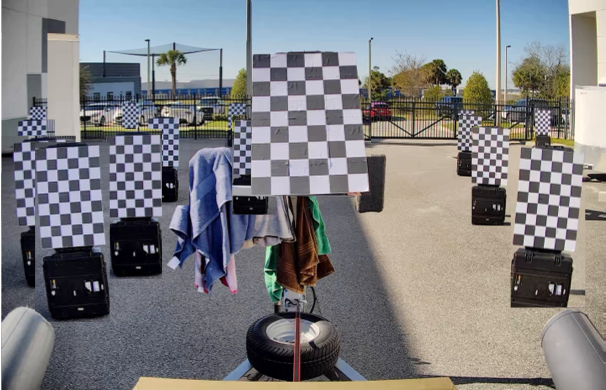
\includegraphics[width=\textwidth]{Images/checkerboard.png}
    \caption{Composite image of checkerboard locations during calibration as seen by the HDR camera}
    \label{fig:chkrbds_vision}
\end{subfigure}
\hfill
\begin{subfigure}[t]{0.45\textwidth}
    \centering
    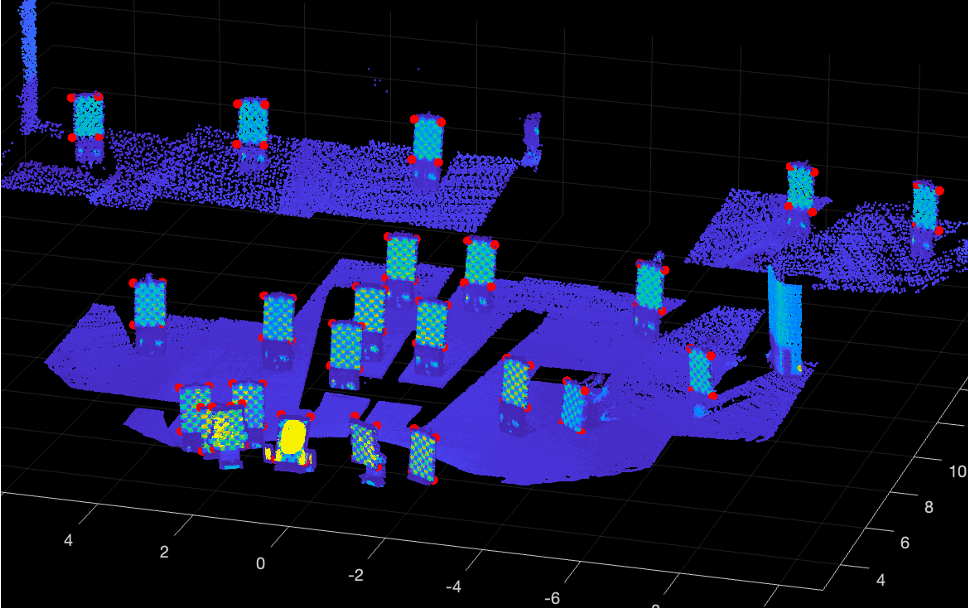
\includegraphics[width=\textwidth]{Images/lidar_calib.png}
    \caption{Composite image of the same checkerboard locations as seen by LiDAR}
    \label{fig:chkrbds_lidar}
\end{subfigure}
\caption{Comparative visualization of checkerboard co-location as seen by visual and LiDAR modality}
\label{fig:camera_calib}
\end{figure}

\begin{figure}[htbp]
    \centering
    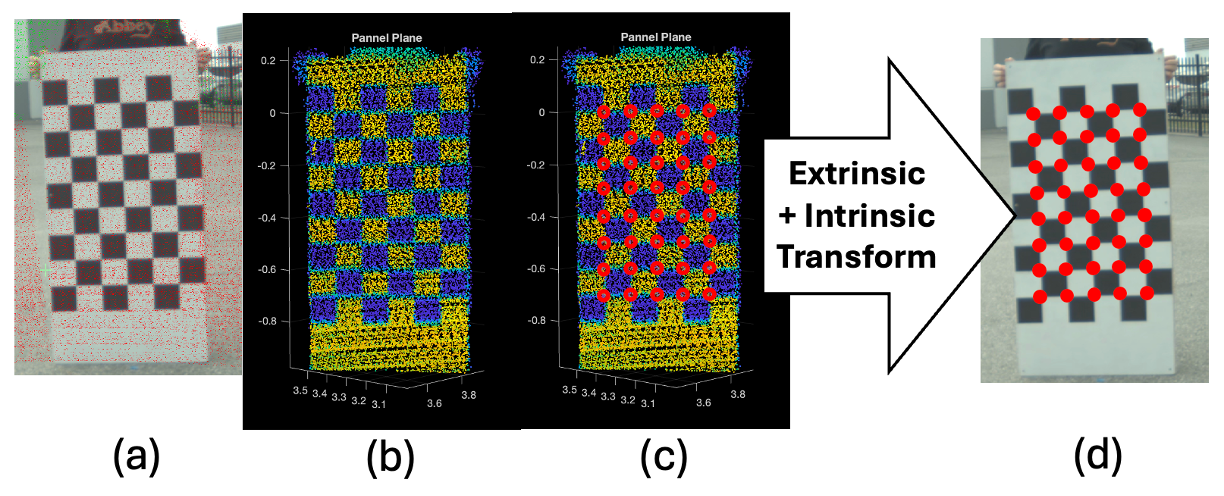
\includegraphics[width=0.9\textwidth]{Images/transform.png}
    \caption{caption}
    \label{fig:lidar_cam_calibration}
\end{figure}

            
\subsubsection{Camera Extrinsics}

For camera-to-LiDAR calibration, the checkerboard calibration dataset is reused from the camera intrinsic calibration.
One second of LiDAR scan data is isolated for each position of the checkerboard pattern to obtain a more dense point cloud and then loaded into the Lidar Calibration tool within MATLAB.
% Data from sensor pairs (e.g. the port viewing LiDAR is paired with the port viewing 4k camera, and the center LiDAR is paired with center 4k and center HDR cameras) are loaded into MATLAB using the Lidar Calibration application.
This function co-locates the three-dimensional checkerboard pattern from the image frame using the identified camera intrinsics and the point cloud data and then estimates the transform between them. 
This function identifies the inner corners of the checkerboard, co-locates this information in the camera and LiDAR frames, and estimates the transform between them \textcolor{blue}{The MathWorks, Inc. (2024). Computer Vision Toolbox version: 24.1 (R2024a)}. 
This initial calibration is shown in Figure \ref{fig:lidar_cam_calibration} by projecting the inner checkerboard corners detected in the images (red) into the LiDAR point cloud data.
While imperfect, this process provides a good first estimate of the extrinsic transformation between the HDR camera frame and LiDAR sensor frame.

\begin{figure}[htbp]
    \centering
    \begin{subfigure}{0.85\textwidth}
        \centering
        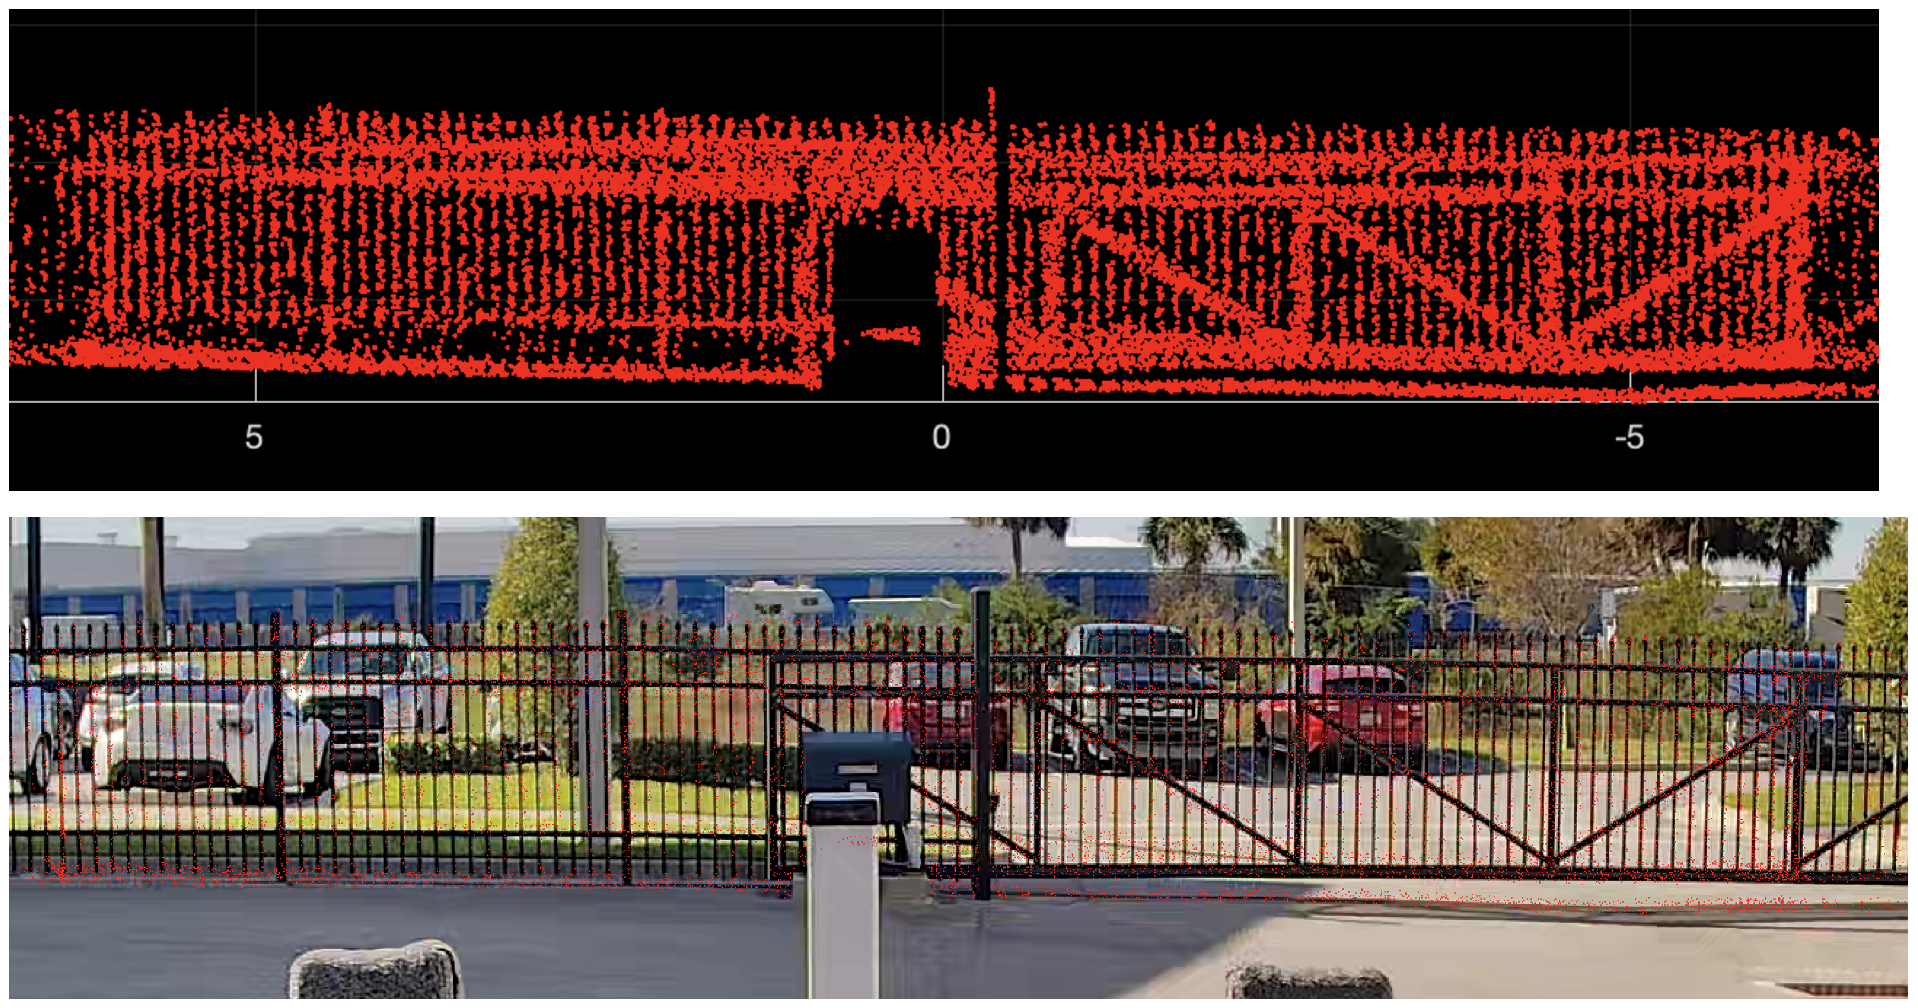
\includegraphics[width=\textwidth]{Images/LiDAR_calib_fence.png}
        \caption{Isolated LiDAR points of fencing (top) projected as red pixels onto the image frame (bottom).}
        \label{fig:LiDAR_calib_fence}
    \end{subfigure}
    
    \vspace{0.5em} % small vertical space between images

    \begin{subfigure}{0.85\textwidth}
        \centering
        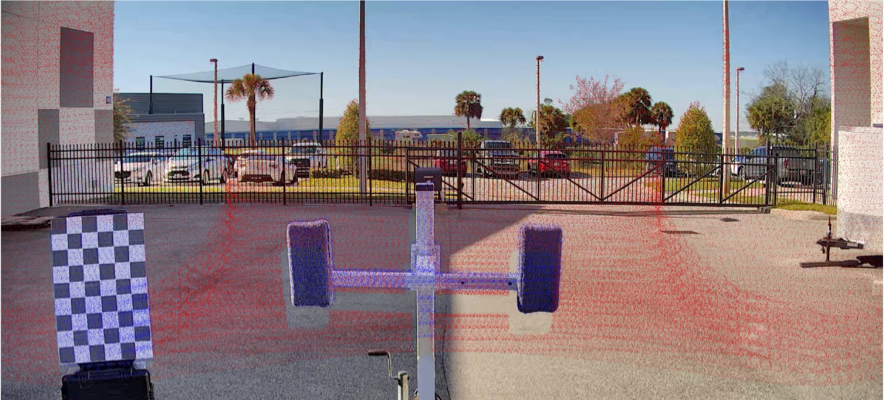
\includegraphics[width=\textwidth]{Images/LiDAR_calib_composite.png}
        \caption{LiDAR points projected onto the image frame as red pixels, with isolated foreground object points in blue}
        \label{fig:LiDAR_calib_composite}
    \end{subfigure}

    \caption{Manual refinement of Camera to LiDAR frame extrinsic transform evaluated by aligning isolated object points within the image frame.}
    \label{fig:LiDAR_calib_combined}
\end{figure}

These initial values are refined through a manual process by projecting LiDAR data onto the image frame and inspecting how the LiDAR points align with objects within the \ac{FOV} such as walls, trees, fencing, and lamp posts, as shown in Figures~\ref{fig:LiDAR_calib_fence} and~\ref{fig:LiDAR_calib_composite}.
The final extrinsic transform is provided in Table~\ref{tbl:extrinsic}.

            
\subsubsection{Livox Extrinsics}
To identify object positions in a different reference frame than it is measured requires an extrinsic transform between the frames. 
This transform defines the translation and rotation (yaw, pitch, roll, $x,y,z$) to make one frame match another and is represented by quaternions or Euler angles.
For Minion, an extrinsic transform is used between the port and starboard facing Livox devices to the central forward facing Livox to create a unified point cloud. Each camera also receives an extrinsic transform to the Livox reference frame.
A flowchart of these transforms is provided in Figure \ref{transform_diagm}.
% required between the center Livox frame and each of the four camera sensors as well as the port and starboard Livox devices.
% Each sensor is calibrated to an $x$-up, $z$-forward, $z$-down reference frame located at the origin of the forward-facing center Livox Horizon, see \ref{transform_diagm}. 

% Each Livox Horizon is equipped with a inertial measurement unit (IMU) to ensure that the final reference frame is level.

% A similar 
% A series of LiDAR scans are simultaneously captured with video from each camera.
% Objects are accurately located within the data sets of both sensor types to perform the spatial calibration between them.

LiDAR-to-LiDAR calibration is performed with first-party software Livox Viewer, available through the manufacturer's website.
This software provides a real-time view of the LiDAR returns and adjustment of the extrinsic calibration for each sensor.
The large flat surfaces of the laboratory, as well as the larger paved area behind the laboratory, both provide excellent large and flat surfaces that allow them to be easily co-located by manually adjusting the extrinsic values.
As shown in Fig~\ref{transform_diagm}, the port and starboard Livox Horizons are transformed into the \textcolor{blue}{center livox} frame, and the extrinsic transforms required to do so are stored in the non-volatile memory of each sensor. This means that once calibrated, the raw point cloud data from each sensor is transmitted in the \textcolor{blue}{center livox} frame.




\begin{table}[ht]
\caption{Final Transforms to Center Livox frame}
\label{extrinsics}
\centering
\begin{tabular}{l|cccccc}
% \hline
Sensor &  roll & pitch & yaw & $x$ & $y$ & $z$\\
\hline \hline 
Livox (port)  & -4.14 & 1.47 & 42.97 & -0.057 & 0.169 & 0\\ \hline
% Livox (fwd) & 0 & 1.63 & 0 & 0 & 0 & 0\\ \hline
Livox (stbd) & 4.25 & 1.85 & -42.6 & -0.057 & -0.169 & 0\\ \hline
\hline

% 4K (port) &  -88.35 &   0.84 & -97.16 & -0.031 & 0.155 & 0.159\\ \hline
HDR (fwd) & 103.85 & -0.69 & 88.83 & -0.032 &0.115 & 0.098\\ \hline
% 4K (fwd) & -88.31&    0.98&  -97.33& -0.023 & 0.095& 0.19\\ \hline
% 4K (stbd) & -88.35&    0.84&  -97.16 & -0.32 & 0.15& 0.16\\ \hline
\end{tabular} \label{tbl:extrinsic}
\end{table}
            
        \subsection{Synchronization} \label{sync}
        
            \subsubsection{Clock Synchronization} \label{clock_sync}

Accurate temporal alignment of observations from multiple sensors operating with independent clocks requires that all sensors share a common time reference. The Minion autonomous surface vessel implements a hierarchical clock synchronization architecture that distributes GPS-disciplined time from a single authoritative source through a cascade of increasingly precise synchronization protocols. This multi-tier approach balances the accuracy requirements of different sensor types---millisecond-level precision for camera frames versus microsecond-level precision for LiDAR points---while maintaining architectural simplicity and operational reliability.
% The time distribution system employs a three-tier hierarchy: GPS Time →\rightarrow
% → \ac{NTP} Distribution →\rightarrow
% → \ac{PTP} Distribution. 
The Pinpoint GPS/INS receiver extracts time from GNSS satellite signals, providing UTC time with typical accuracy of 10--100 nanoseconds. Operating at IP address 201.7.90.30 on the vessel LAN, the GPS unit functions as a stratum-1 \ac{NTP} server, indicating direct attachment to a reference clock. One Atlas PC (Minion A or Minion B) synchronizes its system clock to the Pinpoint GPS via Network Time Protocol using the Chrony daemon, then operates as an \ac{NTP} server for other platform computing resources. The Atlas PC maintains synchronization accuracy typically within 1--10 milliseconds of GPS time, limited primarily by network latency rather than GPS accuracy. The NVIDIA Jetson Xavier camera enclosure computer synchronizes to the Atlas \ac{NTP} server, inheriting GPS-disciplined time for video frame timestamping.

The cascaded architecture ensures that all sensors reference the same GPS time source despite employing different synchronization protocols optimized for their respective accuracy requirements.
\ac{NTP} provides adequate accuracy ($1-10$ ms) for video frame timestamps given the $10$ Hz sampling rate, while LiDAR sensors demand substantially higher timing precision. 
Each Livox Horizon unit incorporates IEEE 1588 \ac{PTP} support for sub-microsecond clock synchronization, with the Jetson Xavier functioning as the \ac{PTP} grandmaster. 
The Linux \ac{PTP} project's \texttt{ptp4l} daemon executes on the Jetson Xavier, broadcasting \ac{PTP} timing packets over the camera enclosure Ethernet network segment that includes the three Livox sensors. 
\ac{PTP} achieves microsecond-level accuracy (typically $1-10 \mu s$) through hardware-timestamped network packets and symmetric delay compensation, meeting the stringent timing requirements for spatial measurement sensors. 
Both the Jetson Xavier and Livox Horizon sensors employ network interfaces with hardware timestamp support, enabling the symmetric delay measurement required for accurate \ac{PTP} synchronization.

To prevent recording with uncalibrated timestamps, the video encoding pipeline implements mandatory synchronization verification before launching camera capture processes. The startup script executes two checks with defined timeouts: first, a 60-second verification that Chrony synchronization is established with ``Normal'' leap status and active connection to the upstream \ac{NTP} source; second, a 30-second confirmation that the system clock reflects actual calendar time rather than a default epoch value. Only after both checks pass does the startup script launch the GStreamer video encoding pipelines, preventing the collection of video data with incorrect temporal references that would compromise subsequent sensor fusion analysis.
            
\subsubsection{Video Pipeline} \label{video pipeline}
            
The video processing pipeline implements a sophisticated timestamp embedding methodology that preserves GPS-synchronized timing information through the entire encoding, transmission, decoding, and recording chain. This approach embeds absolute system timestamps directly into the H.264/H.265 video bitstream as Supplemental Enhancement Information \ac{SEI} metadata, ensuring that timing information remains inseparably bound to the corresponding video frames throughout all processing stages.
Standard video processing workflows typically assign timestamps relative to stream start time, which proves inadequate for multi-sensor fusion applications requiring absolute temporal references. The GStreamer multimedia framework, employed for video capture and encoding, operates with timestamps measured from the beginning of each stream---a convention suitable for multimedia playback synchronization but incompatible with the requirement to associate video frames with LiDAR observations timestamped in GPS time. Several approaches for associating absolute timestamps with video frames were evaluated, including external CSV logging, \ac{RTP} timestamp modification, and visible video overlays. The in-band metadata approach via \ac{SEI} \ac{NAL} units was selected based on critical advantages: timestamps persist through network network transmission; each frame carries its own embedded timestamp with no possibility of misalignment; \ac{SEI} messages comply with H.264/H.265 specifications, making them invariant to video encoding software versions, as well as not requiring custom metadata.
The video encoding pipeline executes on the NVIDIA Jetson Xavier, exploiting hardware-accelerated video encoding engines to achieve real-time compression of the HDR video stream. The GStreamer pipeline structure for each camera follows the sequence listed in~\ref{vide_encode}: 

\begin{algorithm}
\caption{Transmit Pipeline (Jetson Xavier)}
\begin{algorithmic}[1]
\State \texttt{v4l2src (camera capture)}
\State $\rightarrow$ \texttt{capsfilter (video/x-raw, 2880x1860, 25 fps)}
\State $\rightarrow$ \texttt{[timestamp capture probe: sample GPS-sync system time]}
\State $\rightarrow$ \texttt{videoconvert (color space conversion)}
\State $\rightarrow$ \texttt{videorate (downsample to 5 fps)}
\State $\rightarrow$ \texttt{capsfilter (video/x-raw, 2880x1860, 5 fps)}
\State $\rightarrow$ \texttt{x264enc / x265enc (hardware-accelerated compression)}
\State $\rightarrow$ \texttt{[SEI insertion probe: embed timestamp as NAL unit]}
\State $\rightarrow$ \texttt{rtph264pay / rtph265pay (RTP packetization)}
\State $\rightarrow$ \texttt{RTSP server (network transmission)}
\end{algorithmic} \label{vide_encode}
\end{algorithm}

\begin{algorithm}
\caption{Receive Pipeline (Atlas PC)}
\begin{algorithmic}[1]
\State \texttt{udpsrc (UDP network reception, port 5603)}
\State $\rightarrow$ \texttt{rtph264depay / rtph265depay (RTP depacketization)}
\State $\rightarrow$ \texttt{h264parse / h265parse (bitstream parsing)}
\State $\rightarrow$ \texttt{[SEI extraction probe: recover embedded timestamp]}
\State $\rightarrow$ \texttt{avdec\_h264 / avdec\_h265 (software decoding)}
\State $\rightarrow$ \texttt{videoconvert (format conversion)}
\State $\rightarrow$ \texttt{videoscale (optional resolution scaling)}
\State $\rightarrow$ \texttt{appsink (application callback)}
\State $\rightarrow$ \texttt{ROS sensor\_msg/Image publication}
\end{algorithmic} \label{video_decode}
\end{algorithm}

This architecture captures the timestamp as close to image frame capture as possible, and holds the information until after the video is down-sampled and encoded.
A custom GStreamer metadata system propagates absolute timestamps through the processing pipeline. A pad probe attached to the source pad of \texttt{v4l2src} captures system time for each incoming video buffer using \texttt{gettimeofday()}, sampling the \ac{NTP}-synchronized system clock to obtain GPS-disciplined time. The resulting timestamp is attached to the GStreamer buffer as custom metadata that persists through subsequent pipeline elements. When the \texttt{videorate} element reduces the 25 fps input to 5 fps output, the metadata transform callback ensures that the timestamp from the selected buffer is copied to the output frame, preserving the original capture time even when frames are dropped.
The H.264 video compression standard defines \ac{SEI} as a mechanism for carrying metadata alongside compressed video. 
The timestamp \ac{SEI} message employs the unregistered user data payload type (type 5), consisting of the timestamp (8 bytes) encoded as a \texttt{uint64\_t} value representing milliseconds since Unix epoch, followed by 8 bytes of padding to complete a 16-byte payload. 
A pad probe attached to the source pad of the H.264 video encoder (\texttt{nvv4l2h264enc}) constructs and inserts \ac{SEI} \ac{NAL} units before each encoded frame.  
The \ac{SEI} \ac{NAL} unit is prepended to the encoded frame buffer, maintaining the association between timestamp and image content through all subsequent processing stages including \ac{RTP} packetization and \ac{UDP} transmission.

Video transmission from the Jetson to Atlas employs \ac{RTSP} over \ac{UDP} to minimize latency and avoid transmission delays associated with TCP acknowledgment mechanisms. The Atlas PC receives and decodes the \ac{RTSP} streams through a complementary GStreamer pipeline into ROS image messages. A pad probe attached to the H.264/H.265 parser element extracts embedded timestamps from \ac{SEI} \ac{NAL} units before decoding. Due to potential fragmentation of \ac{NAL} units across GStreamer buffers, the extraction implementation accumulates incoming data until complete \ac{NAL} units can be identified and parsed. The extraction logic identifies \ac{SEI} \ac{NAL} units by type, verifies the custom UUID, and extracts the 8-byte timestamp value.

The \texttt{appsink} element at the end of the receive pipeline provides decoded video frames to the application. A callback function executes for each frame, extracting the frame data and publishing it as a ROS \texttt{sensor\_msg/Image} message with the previously extracted \ac{SEI} timestamp converted from millisecond Unix epoch time to ROS time format. 
% The ROS \texttt{image\_transport} package provides efficient image message publication with automatic transport plugin support, creating raw and compressed image topics. 
% Critically, the \ac{SEI}-derived timestamp is applied to all transport variants, ensuring temporal accuracy regardless of which compressed format is recorded.
The video pipeline achieves real-time performance encoding three simultaneous 2880$\times$1860 pixel camera streams at 10 fps with measured end-to-end latency averaging 127 milliseconds from frame capture to ROS publication. Hardware encoding latency ranges from 10--30 ms per frame for H.264/H.265, with network transmission latency of 1--5 ms over the Gigabit LAN and negligible \ac{SEI} insertion overhead (<1 ms). Zero frame drops and zero frame repetition under normal operation confirm the temporal stability of the implementation. The timestamps embedded via \ac{SEI} reflect the GPS-synchronized system clock on the Jetson Xavier at the moment of frame capture, with accuracy depending on the \ac{NTP} synchronization quality between Jetson and Atlas PC, typically achieving 1--10 millisecond accuracy relative to GPS time.
            
            \subsubsection{Temporal Drift} \label{temporal_drift}
            
    \section{Data Output}

\chapter{Dataset} \label{dataset}

\chapter{Real-time Object Detection} \label{object-detection}

    \section{YOLOv8} \label{yolo}

    \section{GB-CACHE} \label{gbcache}

\chapter{Late Fusion}

\chapter{Conclusions}

% This chapter will synthesize findings from all three research objectives:
% - Summary of comparative performance results between LiDAR and vision systems
% - Calibration and synchronization framework effectiveness
% - Real-time processing capability validation
% - Implications for ASV perception system design
% - Contribution to maritime autonomous systems knowledge

\section{Research Objective Achievement Summary}
% Placeholder for objective completion summary

\section{Performance Comparison Findings}
% Placeholder for key comparative analysis conclusions

\section{Implications for ASV System Design}
% Placeholder for practical design guidance conclusions

\chapter{Recommendations and Future Work}

% This chapter will address:
% - Recommendations for ASV perception system design based on findings
% - Sensor selection guidance for maritime applications
% - Future research directions for maritime sensor fusion
% - Technology transfer opportunities to operational systems

\section{ASV Perception System Design Recommendations}
% Placeholder for design guidance recommendations

\section{Future Research Directions}
% Placeholder for future work recommendations

\section{Technology Transfer Opportunities}
% Placeholder for practical application recommendations




% \printbibliography
\bibliographystyle{plainnat}
% \bibliography{References}
\bibliography{Dissertation}

\backmatter

\chapter{A Test of the Appendix System}

% Tables of Results

% \chapter{Another Test of the Appendix System}
% Supplemental Figures.
\end{document}

